\chapter{Overview}\label{ch:overview}
The analog circuit synthesis tool ({\bf acst}) supports following functionalities:

\begin{itemize}
	\item Recognition of basic structures in analog circuits ({\em Structure Recognition}) \cite{Massier2008}
	\item Developing rule sets for new structures to automatically recognize them in circuits ({\em Rule Generation}) \cite{Date2021}
	\item Partitioning of op-amps into their functional blocks ({\em Partitioning }) \cite{ABNG20}
	\item Sizing of basic op-amps ({\em Automatic Sizing}) \cite{ABNG20c}
	\item Synthesis of basic op-amps ({\em Synthesis}) \cite{ICCAD,ABNG20d}
	\item Automatic generation of a topology library currently featuring around 4000 op-amps ({\em Topology Library Generation})
\end{itemize}

\section{Structure Recognition}\label{sec:OverviewStructureRecognition}
The structure recognition methods is able to recognize basic structures as current mirrors and differential pairs in op-amps. It is detailed described in \cite{Massier2008, Massier2010}.

\section{Rule Generation}\label{sec:OverviewRuleGeneration}
The rule generation functionality allows to automatically develop recognition rules for new structures in analog circuits that repeatedly occur like level shifters. The structures are stored in  defined  libraries which can be used to analyze circuits for this structures. The method is described in  \cite{Date2021}.

\section{Partitioning}\label{sec:OverviePartitioning}
The partitioning method automatically recognizes functional blocks in op-amps. These functional blocks are the amplification stages, their subblocks (load, transconductor, stage bias), the op-amp bias circuits, and basic compensation structures. A list of  supported example circuits which can be partitioned is given in Appendix \ref{app:ExampleOpAmps}.
The method is described in detail in \cite{ABNG20}.


\section{Automatic Sizing}\label{sec:OverviewAutomaticSizing}
The automatic sizing method generates initial device sizes for provided analog op-amps. A list of  supported example circuits is given Appendix \ref{app:ExampleOpAmps}.
The method is described in detail in \cite{ABNG20c}.

\section{Synthesis}\label{sec:OverviewSynthesis}
The synthesis method  generates a set of op-amp topologies fulfilling a given set of specifications. Three different op-amp types are supported: fully-differential, complementary and single-output. The method is in detail described in \cite{ABNG20d,SMACD}.

\section{Topology Library Generation}\label{sec:OverviewTopologyLibraryGeneration}
The topology library generation method generates all topologies currently supported by the synthesis method within {\bf acst}. These are currently 3912 topologies including single-output op-amps, symmetrical op-amps, and fully-differential op-amps.


\chapter{Compiling and Installing  acst}\label{ch:CompilingAndInstallingAcst}
To be able to compile {\bf acst}, following additional libraries must be provided:
\begin{itemize}
	\item Boost (\url{https://www.boost.org/})
	\item RapidXml (\url{http://rapidxml.sourceforge.net/})
	\item GeCode (\url{https://www.gecode.org/})
\end{itemize}
If not already available on your computer system. Please download the respective libraries from the provided websites and install them (see Appendix \ref{ch:installationGuideSupplementaryLibraries} for further information).

If not provided on your system, you also need the gnu/g++ compiler collection able to handle C++-17 and CMake. They can be obtained with following command:
\begin{lstlisting}[basicstyle=\ttfamily\scriptsize,backgroundcolor={\color{gray!30}}, escapechar=!]
$ sudo apt install build-essential	
\end{lstlisting}

To compile acst, please follow the steps below.
\begin{enumerate}
	\item Download {\bf acst} from git and safe it into a proper directory "$\{file path\}$".
	\item Open {\tt $\{file path\}$/acst/CMakeLists.txt} and adjust the file path for the inclusion of the RapidXml-library and Boost-library:
	
\begin{lstlisting}[basicstyle=\ttfamily\scriptsize,backgroundcolor={\color{gray!30}}, escapechar=!]

...

###
# Find RapidXml
###
list(APPEND CMAKE_INCLUDE_PATH
	 !\textcolor{red}{\{file path to rapidxml directory\}}!
)
find_package(RapidXml REQUIRED)
include_directories(SYSTEM ${RAPIDXML_INCLUDE_DIR})


###
# Find Boost library 
###
set(BOOST_ROOT !\textcolor{red}{\{file path to boost directory\}}!) 

...

\end{lstlisting}
An example of an adequate {\tt CMakeLists.txt} file is given below:

\begin{lstlisting}[basicstyle=\ttfamily\scriptsize,backgroundcolor={\color{gray!30}}, escapechar=!]
	
...
	
###
# Find RapidXml
###
list(APPEND CMAKE_INCLUDE_PATH
	/usr/local/public/include/rapidxml/ 
)
find_package(RapidXml REQUIRED)
include_directories(SYSTEM ${RAPIDXML_INCLUDE_DIR})
	
	
###
# Find Boost library 
###
set(BOOST_ROOT /usr/include/boost_1_48_0) 
	
...
	
\end{lstlisting}
	
	\item Open {\tt $\{file path\}$/acst/cmake/modules/FindGecode.cmake} and adjust the path for the inclusion of the GeCode-library:
	
\begin{lstlisting}[basicstyle=\ttfamily\scriptsize,backgroundcolor={\color{gray!30}}, escapechar=!]
if(NOT GECODE_FEATURES)
	set(GECODE_FEATURES "driver" "flatzinc" "gist" "graph" "int" "iter"  
		"kernel" "minimodel" "scheduling" "search" "set" "support")
endif()

set(GECODE_INCLUDE  !\textcolor{red}{\{file path to the gecode directory\}}!)

if(GECODE_INCLUDE STREQUAL "GECODE_INCLUDE-NOTFOUND")
	
...
	
\end{lstlisting}

An example of an adequate {\tt FindGecode.cmake} file is given below:

\begin{lstlisting}[basicstyle=\ttfamily\scriptsize,backgroundcolor={\color{gray!30}}, escapechar=!]
if(NOT GECODE_FEATURES)
	set(GECODE_FEATURES "driver" "flatzinc" "gist" "graph" "int" "iter"  
		"kernel" "minimodel" "scheduling" "search" "set" "support")
endif()
	
set(GECODE_INCLUDE  /usr/local/public/include/gecode-release-6.2.0)
	
if(GECODE_INCLUDE STREQUAL "GECODE_INCLUDE-NOTFOUND")
	
...
	
\end{lstlisting}

Please check, that the libraryfiles of gecode are in the directory of  the filepath {\tt\textcolor{red}{$\{$file path to the gecode directory$\}$}}, e.g., libgecodedriver.so. The header of the gecode source code, e.g., drivers.hh should be in another subdirectory called "gecode".

If this is not the case and the library files or the header files of gecode are on other filepaths, adeaquate lines in the  {\tt FindGecode.cmake} file must be adopted:

\begin{lstlisting}[basicstyle=\ttfamily\scriptsize,backgroundcolor={\color{gray!30}}, escapechar=!]
foreach(FEATURE ${GECODE_FEATURES})
if(NOT EXISTS ${GECODE_INCLUDE}/gecode/${FEATURE}.hh)
set(MESSAGE "Could not find ${GECODE_INCLUDE}/gecode/${FEATURE}.hh") ## !\textcolor{red}{must be}!
	## !\textcolor{red}{adopted to point to the file path of the gecode header files}!
set(GECODE_INCLUDE "")
break()
endif()
endforeach(FEATURE)

set(GECODE_LIBS "")
foreach(FEATURE ${GECODE_FEATURES})
list(APPEND GECODE_LIBS ${GECODE_INCLUDE}/libgecode${FEATURE}.so) ## !\textcolor{red}{must be}!
	## !\textcolor{red}{adopted to point to the file path of the gecode library files}!
endforeach(FEATURE)

\end{lstlisting}

	
	\item Open {\tt $\{file path\}$/acst/Control/script/acst.sh} and adjust the file path to the GeCode-library:
	
\begin{lstlisting}[basicstyle=\ttfamily\scriptsize,backgroundcolor={\color{gray!30}}, escapechar=?]
#!/bin/bash

export LD_LIBRARY_PATH="?\textcolor{red}{\{file path to acst\}}?:${LD_LIBRARY_PATH}"
export OA_UNSUPPORTED_PLAT=linux_rhel40
${CMAKE_RUNTIME_OUTPUT_DIRECTORY}/acst $@	
\end{lstlisting}

An example of an adequate {\tt acst.sh} file is given below:

\begin{lstlisting}[basicstyle=\ttfamily\scriptsize,backgroundcolor={\color{gray!30}}, escapechar=?]
#!/bin/bash
	
export LD_LIBRARY_PATH="usr/local/public/include/gecode-release-6.2.0:${LD_LIBRARY
_PATH}"
export OA_UNSUPPORTED_PLAT=linux_rhel40
${CMAKE_RUNTIME_OUTPUT_DIRECTORY}/acst $@
\end{lstlisting}

\item Use following Linux commands to compile {\bf acst}:

\begin{lstlisting}[basicstyle=\ttfamily\scriptsize,backgroundcolor={\color{gray!30}}, escapechar=? ]
$ cd {?\textit{file path}?}/acst    #enters the acst directory
$ mkdir build            #creates a new build folder within acst
$ cd build               #enters the new build folder within acst
$ cmake ..               #runs CMake to build generate a buildsystem
$ cd ..                  # returns to the acst folder
$ make -C build          # builds acst into the build-folder
\end{lstlisting}
\end{enumerate}

Please note to run {\bf acst}, {\tt acst.sh} must be made executable. This can be obtained with the following command in the {\tt \{file path\}/acst/build/bin/} directory:
\begin{lstlisting}[basicstyle=\ttfamily\scriptsize,backgroundcolor={\color{gray!30}}, escapechar=? ]
$ chmod a+x acst.sh
\end{lstlisting}


\chapter{Commands}\label{ch:Commands}
{\bf acst} can be best used using command-scripts. Examples of  command-scripts are given in {\tt acst/InputFileExamples/} ordered according to the different methods. To make a new script executable, use the command {\tt chmod a+x \textcolor{red}{\{newScript.sh\}}}.
Detailed explanations of the different commands that can be used to control {\bf acst} are given below.

With {\tt --help} you get general help. I do not know if this help is useful but you can try.

\section{General Commands}\label{sec:generalCommands}
General commands are not method specific. These are:
\begin{lstlisting}[basicstyle=\ttfamily\scriptsize,backgroundcolor={\color{gray!30}}, escapechar=? ]
--log-level-console [DEBUG/TRACE/OFF]  
\end{lstlisting}
{\tt --log-level-console} specifies what is outputted on the console, debug messages [{\tt DEBUG}], nothing [{\tt OFF}], etc.

\begin{lstlisting}[basicstyle=\ttfamily\scriptsize,backgroundcolor={\color{gray!30}}, escapechar=? ]	
--analysis [structrec/rulegen/partitioning/automaticsizing/synthesis/toplibgen]	
\end{lstlisting}
{\tt --analysis} specifies what method is performed, structure recognition [{\tt structrec}], rule generation [{\tt rulegen}], partitioning [{\tt partitioning}], sizing [{\tt automaticsizing}], synthesis \newline [{\tt synthesis}] or topology library generation [{\tt toplibgen}].

\section{Method Specific Commands}\label{sec:functionSpecificCommands}
Additionally to the general commands, also commands specified for the different functionalities of the tool are needed. 

\subsection{Structure Recognition}\label{sec:CommandsStructRec}
Following additional commands are defined for structure recognition:
\\

\begin{lstlisting}[basicstyle=\ttfamily\scriptsize,backgroundcolor={\color{gray!30}}, escapechar=? ]
--circuit-netlist [relative file path to the circuit netlist to be analysis]
\end{lstlisting}
The circuit netlist contains the devices of the circuit and their interconnections. It must have the HSpice-file-format. An example of a circuit netlist  that can be analyzed is given in App.~\ref{sec:inputFileCircuitNetlist}.
\\

\begin{lstlisting}[basicstyle=\ttfamily\scriptsize,backgroundcolor={\color{gray!30}}, escapechar=? ]
--device-types-file [relative file path to the device types file]
\end{lstlisting}
The device-types-file contains information of the devices supported by {\bf acst}. An example is shown in App. \ref{sec:inputFileDeviceTypeFile}.
\\

\begin{lstlisting}[basicstyle=\ttfamily\scriptsize,backgroundcolor={\color{gray!30}}, escapechar=? ]
--hspice-mapping-file [relative file path to the HSpice mapping file]
\end{lstlisting}
As the circuit netlist is written in HSpice-file-format, the corresponding mapping must be provided in a HSpice-mapping-file. An example is shown in App. \ref{sec:InputFileHSpiceMapping}.
\\

\begin{lstlisting}[basicstyle=\ttfamily\scriptsize,backgroundcolor={\color{gray!30}}, escapechar=? ]
--hspice-supplynet-file [relative file path to the supply net file]
\end{lstlisting}
The supply-net-file defines the supply nets in the circuit. They must be named as global nets in the circuit-netlist-file. An example is shown in App. \ref{sec:inputFileSupplyNetFile}.
\\

\begin{lstlisting}[basicstyle=\ttfamily\scriptsize,backgroundcolor={\color{gray!30}}, escapechar=? ]
--xml-structrec-library-file [abosolut file path to the library used for recognition] 
\end{lstlisting}
The library-file defines the basic structures recognizable by {\bf acst}. This library is integrated in {\bf acst}. The file path is: {\tt \{file path to acst\}/acst/StructRec/xml/AnalogLibrary.xml}. An example of the library-file is shown in App. \ref{sec:inputFileLibraryFile}.
\\

\begin{lstlisting}[basicstyle=\ttfamily\scriptsize,backgroundcolor={\color{gray!30}}, escapechar=? ]
--output-file [relative file path to the output file(file is created by program)] 
\end{lstlisting}
The output-file contains all basic structures recognized by {\bf acst} in the circuit netlist. An example is given in App. \ref{sec:OutputFileStructRec}.

In the following, an example of a command script is shown. The example is provided in {\tt acst/InputFileExamples/StructureRecognition/command.sh}.
\begin{lstlisting}[basicstyle=\ttfamily\scriptsize,backgroundcolor={\color{gray!30}}, escapechar=? ]
?\textcolor{red}{\{absolute file path to acst\}}?/acst/build/bin/acst.sh --circuit-netlist input.ckt 
--device-types-file deviceTypes.xcat --hspice-mapping-file HSpiceMapping.xcat 
--hspice-supplynet-file supplyNets.xcat --analysis structrec --output-file output.xml 
--log-level-console DEBUG --xml-structrec-library-file 
?\textcolor{red}{\{absolute file path to acst\}}?/acst/StructRec/xml/AnalogLibrary.xml 

\end{lstlisting}
To run the script, adjust the absolute file path to {\bf acst} in the script.

\subsection{Rule Generation}\label{sec:commandsRuleGeneration}
Following additional commands are defined for the rule generation method:
\\

\begin{lstlisting}[basicstyle=\ttfamily\scriptsize,backgroundcolor={\color{gray!30}}, escapechar=? ]
--circuit-netlist [relative file path to the circuit netlist containing the circuit for 
				which recognition new rules are created]
\end{lstlisting}
The circuit netlist contains the devices of the circuit and their interconnections. It must have the HSpice-file-format. An example of a circuit netlist  for which new rules can be created is given in  in App. \ref{sec:inputFileCircuitNetlist}.
\\

\begin{lstlisting}[basicstyle=\ttfamily\scriptsize,backgroundcolor={\color{gray!30}}, escapechar=? ]
--device-types-file [relative file path to the device types file]
\end{lstlisting}
The device-types-file contains information of the devices supported by {\bf acst}. An example is shown in App. \ref{sec:inputFileDeviceTypeFile}.
\\

\begin{lstlisting}[basicstyle=\ttfamily\scriptsize,backgroundcolor={\color{gray!30}}, escapechar=? ]
--hspice-mapping-file [relative file path to the HSpice mapping file]
\end{lstlisting}
As the circuit netlist is written in HSpice-file-format, the corresponding mapping must be provided in a HSpice-mapping-file. An example is shown in App. \ref{sec:InputFileHSpiceMapping}.
\\

\begin{lstlisting}[basicstyle=\ttfamily\scriptsize,backgroundcolor={\color{gray!30}}, escapechar=? ]
--hspice-supplynet-file [relative file path to the supply net file]
\end{lstlisting}
The supply-net-file defines the supply nets in the circuit. They must be named as global nets in the circuit netlist file. An example is shown in App. \ref{sec:inputFileSupplyNetFile}.
\\

\begin{lstlisting}[basicstyle=\ttfamily\scriptsize,backgroundcolor={\color{gray!30}}, escapechar=? ]
--xml-structrec-library-file [abosolut file path to the library used for recognition] 
\end{lstlisting}
The library-file defines the basic set of structures that is used for rule generation. It must at least contain the array library ({\tt acst/StructRec/xml/Array/ArrayLibrary.xml}). Also other structures can be added to build the basis structures of the new established rules.
\\

\begin{lstlisting}[basicstyle=\ttfamily\scriptsize,backgroundcolor={\color{gray!30}}, escapechar=? ]
--structure-name [name of the structure for which new rules are created] 
\end{lstlisting}
With the structure name, a new library is created containing the old libraries for recognition as well as the new library created for the structure. Also a folder is created containing the rules for the structure as well as its substructures. Examples are provided in App. \ref{sec:OutputFilesRuleGeneration}.

In the following, an example of a command script is shown. The example is provided in {\tt acst/InputFileExamples/RuleGeneration/command.sh}.
\begin{lstlisting}[basicstyle=\ttfamily\scriptsize,backgroundcolor={\color{gray!30}}, escapechar=? ]
?\textcolor{red}{\{absolute file path to acst\}}?/acst/build/bin/acst.sh --log-level-console DEBUG  --analysis 
rulegen --circuit-netlist cascodedSymmetricalCMOSOTA.hspice --xml-structrec-library-file
?\textcolor{red}{\{absolute file path to acst\}}?/acst/InputFileExamples/RuleGeneration/Library.xml 
--hspice-mapping-file HSpiceMapping.xcat --hspice-supplynet-file supplyNets.xcat 
--device-types-file deviceTypes.xcat --structure-name SymmetricalCascodeOpAmp
\end{lstlisting}
To run the script, adjust the absolute file path to {\bf acst} in the script.


\subsection{Partitioning}\label{sec:commandsPartitioning}
Following additional commands are defined for the partitioning method:
\\

\begin{lstlisting}[basicstyle=\ttfamily\scriptsize,backgroundcolor={\color{gray!30}}, escapechar=? ]
--circuit-netlist [relative file path to the circuit netlist to be analysis]
\end{lstlisting}
The circuit netlist contains the devices of the circuit and their interconnections. It must have the HSpice-file-format. An example of a circuit netlist  that can be analyzed is given in App.~\ref{sec:inputFileCircuitNetlist}.
\\

\begin{lstlisting}[basicstyle=\ttfamily\scriptsize,backgroundcolor={\color{gray!30}}, escapechar=? ]
--device-types-file [relative file path to the device types file]
\end{lstlisting}
The device-types-file contains information of the devices supported by {\bf acst}. An example is shown in App. \ref{sec:inputFileDeviceTypeFile}.
\\

\begin{lstlisting}[basicstyle=\ttfamily\scriptsize,backgroundcolor={\color{gray!30}}, escapechar=? ]
--hspice-mapping-file [relative file path to the HSpice mapping file]
\end{lstlisting}
As the circuit netlist is written in HSpice-file-format, the corresponding mapping must be provided in a HSpice-mapping-file. An example is shown in App. \ref{sec:InputFileHSpiceMapping}.
\\

\begin{lstlisting}[basicstyle=\ttfamily\scriptsize,backgroundcolor={\color{gray!30}}, escapechar=? ]
--hspice-supplynet-file [relative file path to the supply net file]
\end{lstlisting}
The supply-net-file defines the supply nets in the circuit. They must be named as global nets in the circuit-netlist-file. An example is shown in App. \ref{sec:inputFileSupplyNetFile}.
\\

\begin{lstlisting}[basicstyle=\ttfamily\scriptsize,backgroundcolor={\color{gray!30}}, escapechar=? ]
--xml-structrec-library-file [abosolut file path to the library used for recognition] 
\end{lstlisting}
The library-file defines the basic structures recognizable by {\bf acst}. This library is integrated in {\bf acst}. The file path is: {\tt \{file path to acst\}/acst/StructRec/xml/AnalogLibrary.xml}. An example of the library-file is shown in App. \ref{sec:inputFileLibraryFile}.
\\

\begin{lstlisting}[basicstyle=\ttfamily\scriptsize,backgroundcolor={\color{gray!30}}, escapechar=? ]
--output-file [relative file path to the output file(file is created by program)] 
\end{lstlisting}
The output-file contains all functional blocks recognized by {\bf acst} in the circuit netlist. This are, e.g., the amplification stages and their subblocks. An example is given in App. \ref{sec:OutputFilePartitioning}.

In the following, an example of a command script is shown. The example is provided in {\tt acst/InputFileExamples/Partitioning/command.sh}.
\begin{lstlisting}[basicstyle=\ttfamily\scriptsize,backgroundcolor={\color{gray!30}}, escapechar=? ]
?\textcolor{red}{\{absolute file path to acst\}}?/acst/build/bin/acst.sh --log-level-console DEBUG --output-file
cascodedSymmetricalCMOSOTA.xml --circuit-netlist cascodedSymmetricalCMOSOTA.hspice 
--device-types-file deviceTypes.xcat --hspice-mapping-file HSpiceMapping.xcat --analysis 
partitioning --hspice-supplynet-file supplyNets.xcat --xml-structrec-library-file
?\textcolor{red}{\{absolute file path to acst\}}?/acst/StructRec/xml/AnalogLibrary.xml
\end{lstlisting}
To run the script, adjust the absolute file path to {\bf acst} in the script.


\subsection{Automatic Sizing}\label{sec:commandsAutomaticSizing}
Following additional commands are defined for automatic sizing:
\\

\begin{lstlisting}[basicstyle=\ttfamily\scriptsize,backgroundcolor={\color{gray!30}}, escapechar=? ]
--circuit-netlist [relative file path to the circuit netlist to be analysis]
\end{lstlisting}
The circuit netlist contains the devices of the circuit to be sized and their interconnections. It must have the HSpice-file-format. An example of a circuit netlist that can be sized is given in App. \ref{sec:inputFileCircuitNetlist}. 
\\

\begin{lstlisting}[basicstyle=\ttfamily\scriptsize,backgroundcolor={\color{gray!30}}, escapechar=? ]
--device-types-file [relative file path to the device types file]
\end{lstlisting}
The device-types-file contains information of the devices supported by {\bf acst}. An example is shown in App. \ref{sec:inputFileDeviceTypeFile}.
\\

\begin{lstlisting}[basicstyle=\ttfamily\scriptsize,backgroundcolor={\color{gray!30}}, escapechar=? ]
--hspice-mapping-file [relative file path to the HSpice mapping file]
\end{lstlisting}
As the circuit netlist is written in HSpice-file-format, the corresponding mapping must be provided in a HSpice-mapping-file. An example is shown in App. \ref{sec:InputFileHSpiceMapping}.
\\

\begin{lstlisting}[basicstyle=\ttfamily\scriptsize,backgroundcolor={\color{gray!30}}, escapechar=? ]
--hspice-supplynet-file [relative file path to the supply net file]
\end{lstlisting}
The supply-net-file defines the supply nets in the circuit. They must be named as global nets in the circuit-netlist-file. An example is shown in App. \ref{sec:inputFileSupplyNetFile}.
\\

\begin{lstlisting}[basicstyle=\ttfamily\scriptsize,backgroundcolor={\color{gray!30}}, escapechar=? ]
--xml-structrec-library-file [abosolute file path to the library used for recognition] 
\end{lstlisting}
The library-file defines the basic structures recognizable by {\bf acst}. This library is integrated in {\bf acst}. The file path is: {\tt \{file path to acst\}/acst/StructRec/xml/AnalogLibrary.xml}. An example of the library-file is shown in App. \ref{sec:inputFileLibraryFile}.
\\

\begin{lstlisting}[basicstyle=\ttfamily\scriptsize,backgroundcolor={\color{gray!30}}, escapechar=? ]
--xml-technologie-file [relative file path to the technology file] 
\end{lstlisting}
The technology-file contains all parameters of the manufacturing process needed in the sizing algorithm. An example how it must look like and which parameters are needed is given in App. \ref{sec:inputFileTechnologyFile}.

\begin{lstlisting}[basicstyle=\ttfamily\scriptsize,backgroundcolor={\color{gray!30}}, escapechar=? ]
--xml-circuit-information-file [relative file path to the circuit information file] 
\end{lstlisting}
The circuit-information-file contains all parameters and specifications to the circuit performance. An example how it must look like and which parameters and specifications are needed is given in App. \ref{sec:inputFileCircuitParametersAndSpecifications}.

\begin{lstlisting}[basicstyle=\ttfamily\scriptsize,backgroundcolor={\color{gray!30}}, escapechar=? ]
--transistor-model [SHM/EKV] 
\end{lstlisting}
{\tt --transistor-model} specifies which transistor model is used by the sizing algorithm, Shichmann-Hodge model [{\tt SHM}], EKV-model (currently not supported) [{\tt EKV}].

\begin{lstlisting}[basicstyle=\ttfamily\scriptsize,backgroundcolor={\color{gray!30}}, escapechar=? ]
--scaling [0.1mum/1mum] 
\end{lstlisting}
{\tt --scaling} specifies with which discretization the device sizes are calculated, with an accuracy of 0.1 mum [{\tt 0.1mum}], or with an accuracy of 1 mum [{\tt 1mum}].

\begin{lstlisting}[basicstyle=\ttfamily\scriptsize,backgroundcolor={\color{gray!30}}, escapechar=? ]
--runtime [secs] 
\end{lstlisting}
{\tt --runtime} names the time in which the solver has to find solutions for a circuit. Its is provided in secs.


\begin{lstlisting}[basicstyle=\ttfamily\scriptsize,backgroundcolor={\color{gray!30}}, escapechar=? ]
--output-file [relative file path to the output file(file is created by program)] 
\end{lstlisting}
The output-file contains all device sizes calculated by the program, the estimated performance values and the voltage and current values for the circuit in the dc-operation point. An example is given in App. \ref{sec:OutputFileAutomaticSizing}.

In the following, an example of a command script is shown. The example is provided in {\tt acst/InputFileExamples/AutomaticSizing/command.sh}.
\begin{lstlisting}[basicstyle=\ttfamily\scriptsize,backgroundcolor={\color{gray!30}}, escapechar=? ]
?\textcolor{red}{\{absolute file path to acst\}}?/acst/build/bin/acst.sh --log-level-console DEBUG --analysis 
automaticsizing --circuit-netlist cascodedSymmetricalCMOSOTA.hspice --output-file 
cascodedSymmetricalCMOSOTA.xml --hspice-mapping-file HSpiceMapping.xcat --scaling 0.1mum
--transistor-model SHM --device-types-file deviceTypes.xcat --xml-structrec-library-file 
?\textcolor{red}{\{absolute file path to acst\}}?/acst/StructRec/xml/AnalogLibrary.xml --hspice-supplynet-file
supplyNets.xcat --xml-technologie-file TechnologieFile.xml --runtime 5
--xml-circuit-information-file CircuitParameterAndSpecifications.xml 
\end{lstlisting}
To run the script, adjust the absolute file path to {\bf acst} in the script.

\subsection{Synthesis}\label{sec:commandsSynthesis}
Two types of circuit synthesis can be performed. A synthesis featuring a  topology library with around 4000 topologies and a synthesis featuring a smaller topology library with 36 topologies. While in the synthesis process with 4000 topologies, the topologies are dynamically generated, the synthesis with only 36 topologies has a fixed HSpice library.

Which library is used is defined by following command:
\begin{lstlisting}[basicstyle=\ttfamily\scriptsize,backgroundcolor={\color{gray!30}}, escapechar=? ]
--use-hspice-library [true/false]
\end{lstlisting}
When {\tt --use-hspice-library} is set to {\tt true} the smaller HSpice-library is used otherwise the large library is used.
\\

Other additional command are:
\begin{lstlisting}[basicstyle=\ttfamily\scriptsize,backgroundcolor={\color{gray!30}}, escapechar=? ]
--device-types-file [relative file path to the device types file]
\end{lstlisting}
The device-types-file contains information of the devices supported by {\bf acst}. An example is shown in App. \ref{sec:inputFileDeviceTypeFile}.
\\

\begin{lstlisting}[basicstyle=\ttfamily\scriptsize,backgroundcolor={\color{gray!30}}, escapechar=? ]
--xml-structrec-library-file [abosolute file path to the library used for recognition] 
\end{lstlisting}
The library-file defines the basic structures recognizable by {\bf acst}. This library is integrated in {\bf acst}. The file path is: {\tt \{file path to acst\}/acst/StructRec/xml/AnalogLibrary.xml}. An example of the library-file is shown in App. \ref{sec:inputFileLibraryFile}.
\\

\begin{lstlisting}[basicstyle=\ttfamily\scriptsize,backgroundcolor={\color{gray!30}}, escapechar=? ]
--xml-technologie-file [relative file path to the technology file] 
\end{lstlisting}
The technology-file contains all parameters of the manufacturing process needed in the sizing algorithm. An example how it must look like and which parameters are needed is given in App. \ref{sec:inputFileTechnologyFile}.

\begin{lstlisting}[basicstyle=\ttfamily\scriptsize,backgroundcolor={\color{gray!30}}, escapechar=? ]
--xml-circuit-information-file [relative file path to the circuit information file] 
\end{lstlisting}
The circuit-information-file contains all circuit parameters and specifications to the circuit performance. An example how it must look like and which parameters and specifications are needed is given in App. \ref{sec:inputFileCircuitSpecifications}.

\begin{lstlisting}[basicstyle=\ttfamily\scriptsize,backgroundcolor={\color{gray!30}}, escapechar=? ]
--transistor-model [SHM/EKV] 
\end{lstlisting}
{\tt --transistor-model} specifies which transistor model is used by the sizing algorithm, Shichmann-Hodge model [{\tt SHM}], EKV-model (currently not supported) [{\tt EKV}].

\begin{lstlisting}[basicstyle=\ttfamily\scriptsize,backgroundcolor={\color{gray!30}}, escapechar=? ]
--scaling [0.1mum/1mum] 
\end{lstlisting}
{\tt --scaling} specifies with which discretization the device sizes are calculated, with an accuracy of 0.1 mum [{\tt 0.1mum}], or with an accuracy of 1 mum [{\tt 1mum}].

\begin{lstlisting}[basicstyle=\ttfamily\scriptsize,backgroundcolor={\color{gray!30}}, escapechar=? ]
--HSPICE-netlist-dir [path where the files of the circuits fulfilling the specification 
                       are written to]
\end{lstlisting}
For each circuit fulfilling the specifications, a file is created containing the circuit netlist ready to be read in by Cadence \cite{Cadence}. Also, the file lists the expected performance values. An example of such a file is provided in App. \ref{sec:OutputFileSynthesis}.

When the hspice circuit library is used additional command are needed:
\begin{lstlisting}[basicstyle=\ttfamily\scriptsize,backgroundcolor={\color{gray!30}}, escapechar=? ]
--xml-circuit-library-file [absolute file path to the HSpice circuit library]
\end{lstlisting}
The circuit-library-file defines the topologies used in the synthesis algorithm. This library is integrated in {\bf acst}. The file path is: {\tt \{file path to acst\}/acst/Synthesis/hspice/Library.xml}. An example of the library-file is shown in App. \ref{sec:inputFileLibraryFile}.
\\

\begin{lstlisting}[basicstyle=\ttfamily\scriptsize,backgroundcolor={\color{gray!30}}, escapechar=? ]
--hspice-mapping-file [relative file path to the HSpice mapping file]
\end{lstlisting}
As the library is written in HSpice-file-format, the corresponding mapping must be provided in a HSpice-mapping-file. An example is shown in App. \ref{sec:InputFileHSpiceMapping}.
\\

\begin{lstlisting}[basicstyle=\ttfamily\scriptsize,backgroundcolor={\color{gray!30}}, escapechar=? ]
--hspice-supplynet-file [relative file path to the supply net file]
\end{lstlisting}
The supply-net-file defines the supply nets in the circuit. They must be named as global nets in the circuit-netlist-file. An example is shown in App. \ref{sec:inputFileSupplyNetFile}.
\\

In the following, an example of a command script is shown using the large circuit library. The example is provided in {\tt acst/InputFileExamples/Synthesis/command.sh}.
\begin{lstlisting}[basicstyle=\ttfamily\scriptsize,backgroundcolor={\color{gray!30}}, escapechar=? ]
?\textcolor{red}{\{absolute file path to acst\}}?/acst/build/bin/acst.sh --log-level-console DEBUG --analysis 
synthesis --device-types-file deviceTypes.xcat --xml-structrec-library-file
 ?\textcolor{red}{\{absolute file path to acst\}}?/acst/StructRec/xml/AnalogLibrary.xml   --scaling 1mum
--transistor-model SHM --xml-circuit-information-file CircuitSpecifications.xml  
--xml-technologie-file TechnologieFile.xml --HSPICE-netlist-dir 
?\textcolor{red}{\{absolute file path to acst\}}?/acst/InputFileExamples/Synthesis/HspiceNetlist
\end{lstlisting}
To run the script, adjust the absolute file path to {\bf acst} in the script.

The following command script is an example for a script using the small HSpice circuit library. The example is provided in {\tt acst/InputFileExamples/SynthesisSmallLibrary/command.sh}.
\begin{lstlisting}[basicstyle=\ttfamily\scriptsize,backgroundcolor={\color{gray!30}}, escapechar=? ]
?\textcolor{red}{\{absolute file path to acst\}}?/acst/build/bin/acst.sh --log-level-console DEBUG --analysis
synthesis --use-hspice-library true --xml-technologie-file TechnologieFile.xml
--xml-circuit-information-file CircuitSpecifications.xml --xml-structrec-library-file 
?\textcolor{red}{\{absolute file path to acst\}}?/acst/StructRec/xml/AnalogLibrary.xml  --transistor-model SHM 
--xml-circuit-library-file ?\textcolor{red}{\{absolute file path to acst\}}?/acst/Synthesis/hspice/Library.xml 
--hspice-mapping-file HSpiceMapping.xcat --hspice-supplynet-file supplyNets.xcat 
--device-types-file deviceTypes.xcat  --scaling 1mum --HSPICE-netlist-dir
?\textcolor{red}{\{absolute file path to acst\}}?/acst/InputFileExamples/SynthesisSmallLibrary/Netlist 
\end{lstlisting}
To run the script, adjust the absolute file path to {\bf acst} in the script.


\subsection{Topology Library Generation}\label{sec:commandsTopologyLibraryGeneration}
Following additional commands are defined for the topology library generation method:
\\

\begin{lstlisting}[basicstyle=\ttfamily\scriptsize,backgroundcolor={\color{gray!30}}, escapechar=? ]
--HSPICE-netlist-dir [path where the files of the library are written to]
\end{lstlisting}
For each circuit in the library a HSpice-file is created containing the circuit netlist. An example of such a file is provided in App. \ref{sec:OutputFileTopologyLibraryGeneration}.
\\

Adding the structure library to the command with
\begin{lstlisting}[basicstyle=\ttfamily\scriptsize,backgroundcolor={\color{gray!30}}, escapechar=? ]
--xml-structrec-library-file [abosolute file path to the library used for recognition] 
\end{lstlisting}
and the device-type-file with
\begin{lstlisting}[basicstyle=\ttfamily\scriptsize,backgroundcolor={\color{gray!30}}, escapechar=? ]
--device-types-file [relative file path to the device types file]
\end{lstlisting}
leads to a generation of circuit files with labeled transistors. To each transistor, its function in the circuit is written (Fig. \ref{fig:outputFileTopologyGenerationWithTransistorLabels})



In the following, an example of a command script is shown. The example is provided in {\tt acst/InputFileExamples/TopologyLibraryGeneration/command.sh}.
\begin{lstlisting}[basicstyle=\ttfamily\scriptsize,backgroundcolor={\color{gray!30}}, escapechar=? ]
?\textcolor{red}{\{absolute file path to acst\}}?/acst/build/bin/acst.sh --log-level-console DEBUG 
--analysis toplibgen --HSPICE-netlist-dir 
?\textcolor{red}{\{absolute file path to acst\}}?/acst/InputFileExamples/TopologyLibraryGeneration/Netlists
\end{lstlisting}
To run the script, adjust the absolute file path to {\bf acst} in the script.

To generate circuit files with transistor labels, following command script can be used:
\begin{lstlisting}[basicstyle=\ttfamily\scriptsize,backgroundcolor={\color{gray!30}}, escapechar=? ]
?\textcolor{red}{\{absolute file path to acst\}}?/acst/build/bin/acst.sh --log-level-console DEBUG 
--analysis toplibgen --device-types-file deviceTypes.xcat --xml-structrec-library-file 
?\textcolor{red}{\{absolute file path to acst\}}?/acst/StructRec/xml/AnalogLibrary.xml --HSPICE-netlist-dir 
?\textcolor{red}{\{absolute file path to acst\}}?/acst/InputFileExamples/TopologyLibraryGeneration/Netlists
\end{lstlisting}
To run the script, adjust the absolute file path to {\bf acst} in the script.



\chapter{Tests}\label{ch:Tests}

For structure recognition, rule generation and partitioning automatic tests are provided. They can be started in {\tt acst/build/} with the command {\tt ctest}. The results are written to \linebreak {\tt acst/build/Testing/}.


\chapter{Examples}\label{ch:Examples}
Examples for each method are provided in {\tt acst/InputFileExamples/}.

\newpage
\appendix
\chapter{Example Input Files}\label{ch:exampleInputFiles}
In the following, examples of input files to {\bf acst} are provided.

\section{Circuit Netlist}\label{sec:inputFileCircuitNetlist}
The circuit netlist must always be written in HSpice-format. To obtain an error-free recognition of the functional blocks in op-amps, the supply nets of the circuit must be marked as global nets.

\begin{figure}[h]
\begin{lstlisting}[basicstyle=\ttfamily\scriptsize,backgroundcolor={\color{gray!30}}, escapechar=? ]
** Design library name: CascodeSymmetricalCMOSOTA
** Design cell name: cascodeSymmetricalCMOSOTA
** Design view name: schematic
.GLOBAL vdd! gnd!

.TEMP 25.0
.OPTION
+    ARTIST=2
+    INGOLD=2
+    PARHIER=LOCAL
+    PSF=2

** Library name: CascodeSymmetricalCMOSOTA
** Cell name: cascodeSymmetricalCMOSOTA
** View name: schematic
m17 net30 ibias gnd! gnd! nmos
m8 ibias ibias gnd! gnd! nmos
m7 net20 net20 gnd! gnd! nmos
m6 net26 net20 net48 net48 nmos
m5 net48 net26 gnd! gnd! nmos
m4 net40 inp net36 net36 nmos
m3 net29 inn net36 net36 nmos
m2 net42 net26 gnd! gnd! nmos
m1 out net20 net42 net42 nmos
m0 net36 ibias gnd! gnd! nmos
m16 net30 net30 vdd! vdd! pmos
m15 net20 net30 vdd! vdd! pmos
m14 net26 net30 net27 net27 pmos
m13 net40 net40 vdd! vdd! pmos
m12 net27 net29 vdd! vdd! pmos
m11 net29 net29 vdd! vdd! pmos
m10 net44 net40 vdd! vdd! pmos
m9 out net30 net44 net44 pmos
cl out gnd!
.END
\end{lstlisting}
\caption{Example of a circuit netlist file ({\tt acst/InputFileExamples/AutomaticSizing/\protect \linebreak cascodedSymmetricalCMOSOTA.hspice})}
\end{figure}

Rules for the interpretation of the HSpice-file are  set in the HSpice-mapping-file (Sec. \ref{sec:InputFileHSpiceMapping}). The file defines the device naming convention, and the number of pins for specified devices. Also model types are defined. The supply nets defined as global net must be listed in the supply-net-file.

\section{HSpice Mapping File}\label{sec:InputFileHSpiceMapping}
The HSpice-mapping-file defines the interpretation of the circuit-netlist-file. The file defines the device naming convention, and the number of pins for specified devices. Also model types are defined.

\begin{figure}[H]
	\begin{lstlisting}[basicstyle=\ttfamily\scriptsize,backgroundcolor={\color{gray!30}}, escapechar=? ]
<deviceLineMapper>
	<deviceLineMapping identifier ="q">
		<deviceTypeName>Bipolar</deviceTypeName>
		<deviceIdentifier position="0"/>
		<pins>
			<pin pinType="Collector" position="1"/>
			<pin pinType="Base" position="2"/>
			<pin pinType="Emitter" position="3"/>
		</pins>
		<modelName position="5">
			<model name="pnp" techType="p"/>
			<model name="npn" techType="n"/>
		</modelName>    
	</deviceLineMapping>
	<deviceLineMapping identifier ="m">
		<deviceTypeName>Mosfet</deviceTypeName>
		<deviceIdentifier position="0"/>
		<pins>
			<pin pinType="Drain" position="1"/>
			<pin pinType="Gate" position="2"/>
			<pin pinType="Source" position="3"/>
			<pin pinType="Bulk" position="4"/>
		</pins>
		<modelName position="5">
			<model name="pmos" techType="p"/>
			<model name ="pmos4" techType="p"/>
			<model name ="pmos24" techType="p"/>
			<model name="nmos" techType="n"/>
			<model name="nmos4" techType="n"/>
			<model name="nmos24" techType="n"/>
		</modelName>    
	</deviceLineMapping>
	<deviceLineMapping identifier ="c">
		<deviceTypeName>Capacitor</deviceTypeName>
		<deviceIdentifier position="0"/>
		<pins>
			<pin pinType="Plus" position="1"/>
			<pin pinType="Minus" position="2"/>
		</pins>
		<techType>undefined</techType>   
	</deviceLineMapping>
	<deviceLineMapping identifier ="r">
		<deviceTypeName>Resistor</deviceTypeName>
		<deviceIdentifier position="0"/>
		<pins>
			<pin pinType="Plus" position="1"/>
			<pin pinType="Minus" position="2"/>
		</pins>
		<techType>undefined</techType>   
	</deviceLineMapping>
	<deviceLineMapping identifier ="l">
		<deviceTypeName>Inductor</deviceTypeName>
		<deviceIdentifier position="0"/>
		<pins>
			<pin pinType="Plus" position="1"/>
			<pin pinType="Minus" position="2"/>
		</pins>
		<techType>undefined</techType>   
	</deviceLineMapping>
	<deviceLineMapping identifier ="d">
		<deviceTypeName>Diode</deviceTypeName>
		<deviceIdentifier position="0"/>
		<pins>
			<pin pinType="Anode" position="1"/>
			<pin pinType="Cathode" position="2"/>
		</pins>
		<techType>undefined</techType>   
	</deviceLineMapping>
</deviceLineMapping>
\end{lstlisting}
\caption{Example of a HSpice-mapping-file ({\tt acst/InputFileExamples/Automatic\protect \linebreak Sizing/HSpiceMapping.xcat})}
\end{figure}

\section{Supply Net File}\label{sec:inputFileSupplyNetFile}
The supply-net-file list all supply nets supported as global nets. Two different voltage level can be specified.

\begin{figure}[H]
	\begin{lstlisting}[basicstyle=\ttfamily\scriptsize,backgroundcolor={\color{gray!30}}, escapechar=? ]
GND_1 "gnd!"
GND_1 "vss!"
GND_1 "vssb!"
GND_1 "vssp!"
GND_1 "vssb"
GND_1 "vssp"
VDD_1 "vddLow!"
VDD_2 "vdd!"
VDD_2 "vddp!"
VDD_2 "vdd"
VDD_2 "vddp"
VDD_1 "Vdd"
	\end{lstlisting}
	\caption{Example of a supply net file ({\tt acst/InputFileExamples/AutomaticSizing/\protect \linebreak supplyNets.xcat})}
\end{figure}

\section{Device Types File}\label{sec:inputFileDeviceTypeFile}
 The device-types-file defines the devices supported by {\bf acst} and their parameters, as pin names and doping types.

\begin{figure}[H]
	\begin{lstlisting}[basicstyle=\ttfamily\scriptsize,backgroundcolor={\color{gray!30}}, escapechar=? ]
<deviceTypes>
	<deviceType name = "Mosfet">
		<techTypes>
			<techType>n</techType>
			<techType>p</techType>
		</techTypes>
		<pinTypes>
			<pinType>Drain</pinType>
			<pinType>Gate</pinType>
			<pinType>Source</pinType>
			<pinType optional = "true" autoConnection="Source">Bulk</pinType
			   >
		</pinTypes>
	</deviceType>
	<deviceType name = "Bipolar">
		<techTypes>
			<techType>n</techType>
			<techType>p</techType>
		</techTypes>
		<pinTypes>
			<pinType>Emitter</pinType>
			<pinType>Base</pinType>
			<pinType>Collector</pinType>
		</pinTypes>
	</deviceType>
	<deviceType name = "Resistor">
		<techTypes>
			<techType>undefined</techType>
		</techTypes>
		<pinTypes>
			<pinType>Plus</pinType>
			<pinType>Minus</pinType>
		</pinTypes>
	</deviceType>
	<deviceType name = "Capacitor">
		<techTypes>
			<techType>undefined</techType>
		</techTypes>
		<pinTypes>
			<pinType>Plus</pinType>
			<pinType>Minus</pinType>
		</pinTypes>
	</deviceType>
	<deviceType name = "Inductor">
		<techTypes>
			<techType>undefined</techType>
		</techTypes>
		<pinTypes>
			<pinType>Plus</pinType>
			<pinType>Minus</pinType>
		</pinTypes>
	</deviceType>
	<deviceType name = "Diode">
		<techTypes>
			<techType>undefined</techType>
		</techTypes>
		<pinTypes>
			<pinType>Anode</pinType>
			<pinType>Cathode</pinType>
		</pinTypes>
	</deviceType>
</deviceTypes>	
	\end{lstlisting}
	\caption{Example of a device-types-file ({\tt acst/InputFileExamples/AutomaticSizing/\protect \linebreak deviceTypes.xcat})}
\end{figure}

\section{Technology File}\label{sec:inputFileTechnologyFile}
The technology-file contains the parameters of the process used for the manufacturing of the circuit. It is needed for the automatic sizing method and synthesis method.

\begin{figure}[H]
	\begin{lstlisting}[basicstyle=\ttfamily\scriptsize,backgroundcolor={\color{gray!30}}, escapechar=? ]
<general>
   <thermalVoltage Vt = "0.026"></thermalVoltage><!--- [V] -->
</general>
<pmos>
   <thresholdVoltage vth="-0.564"></thresholdVoltage><!--- [V] -->
   <mobilityOxideCapacity muCox="0.00003574"></mobilityOxideCapacity><!--- [A/(V^2)] -->
   <earlyVoltage earlyVoltage="2.86"></earlyVoltage><!--- [V/mum] -->
   <overlapCapacity Cgdov = "0.000000000666" ></overlapCapacity><!--- [F/m] -->
   <gateOxideCapacity Cox = "0.006058"></gateOxideCapacity><!--- [F/m2] --->
   <zeroBiasBulkJunctionCapacitance Cj = "0.001894"></zeroBiasBulkJunctionCapacitance><!
    --- [F/m^2] -->
   <zeroBiasSidewallBulkJunctionCapacitance Cjsw = "0.0000000003626"></zeroBiasSidewall
    BulkJunctionCapacitance><!--- [F/m] -->
   <bulkJunctionContactPotential pb = "0.99"></bulkJunctionContactPotential><!--- [V] 
    -->
   <lateralDiffusionLength Ldiff= "0.0000009968"></lateralDiffusionLength><!-- [mum] -->
   <slopeFactor n="1.31"></slopeFactor>
   <channelLengthCoefficientStrongInversion lamda="0.029"></channelLengthCoefficientStro
    ngInversion>
   <channelLengthCoefficientWeakInversion lamda="0.074"></channelLengthCoefficientWeakIn
    version>
   <minArea Amin="10"></minArea><!--- [mum^2] -->
   <minLength Lmin="1"></minLength><!--- [mum] --><!--- Is used as integer in the p
    rogram -->
   <minWidth Wmin="1"></minWidth><!--- [mum] --><!--- Is used as integer in the program 
    -->
</pmos>
<nmos>
   <thresholdVoltage vth="0.405"></thresholdVoltage><!--- [V] -->
   <mobilityOxideCapacity muCox="0.0001693"></mobilityOxideCapacity><!--- [A/(V^2)] -->
   <earlyVoltage earlyVoltage="4.4"></earlyVoltage><!--- [V/mum] -->
   <overlapCapacity Cgdov = "0.000000000620" ></overlapCapacity><!--- [F/m] -->
   <gateOxideCapacity Cox = "0.006058"></gateOxideCapacity><!--- [F/m2] --->
   <zeroBiasBulkJunctionCapacitance Cj = "0.001812"></zeroBiasBulkJunctionCapacitance><!
   --- [F/m^2] -->
   <zeroBiasSidewallBulkJunctionCapacitance Cjsw = "0.0000000005341"></zeroBiasSidewallB
    ulkJunctionCapacitance><!--- [F/m] -->
   <bulkJunctionContactPotential pb = "0.5"></bulkJunctionContactPotential><!--- [V] -->
   <lateralDiffusionLength Ldiff= "0.00003162"></lateralDiffusionLength><!-- [mum] -->
   <slopeFactor n="1.75"></slopeFactor>
   <channelLengthCoefficientStrongInversion lamda="0.024"></channelLengthCoefficientStro
    ngInversion>
   <channelLengthCoefficientWeakInversion lamda="0.07"></channelLengthCoefficientWeakInv
    ersion>
   <minArea Amin="10"></minArea><!--- [mum] -->
   <minLength Lmin="1"></minLength><!--- [mum] --><!--- Is used as integer in the progra
    m -->
   <minWidth Wmin="1"></minWidth><!--- [mum] --><!--- Is used as integer in the program 
    -->
</nmos>	
	\end{lstlisting}
	\caption{Example of a technology-file ({\tt acst/InputFileExamples/AutomaticSizing/\protect \linebreak TechnologyFile.xml})}
\end{figure}

\section{Circuit Parameters and Specifications}\label{sec:inputFileCircuitParametersAndSpecifications}
The circuit-parameters-and-specifications-file contains all information about the circuit needed for circuit sizing. It is needed for the automatic sizing method. 
\begin{figure}[H]
	\begin{lstlisting}[basicstyle=\ttfamily\scriptsize,backgroundcolor={\color{gray!30}}, escapechar=? ]
<CircuitParameter>
   <LoadCapacities>
      <LoadCapacity>
         <Value>20</Value><!--- [pF] -->
         <DeviceName>cl</DeviceName>
      </LoadCapacity>
   </LoadCapacities>
   <SupplyVoltagePin>
      <SupplyVoltage Vdd="5"></SupplyVoltage><!--- [V] -->
      <NetName>vdd!</NetName>
   </SupplyVoltagePin>
   <GroundPin>
      <GroundVoltage Gnd="0"></GroundVoltage><!--- [V] -->
      <NetName>gnd!</NetName>
   </GroundPin>
   <CurrentBiasPin>
     <BiasCurrent Ibias="10"></BiasCurrent><!--- [uA] -->
     <NetName>ibias</NetName>
   </CurrentBiasPin>
   <InputPinMinus>
      <InputVoltage Vin="2.5"></InputVoltage><!--- [V] -->
      <NetName>inn</NetName>
   </InputPinMinus>
   <InputPinPlus>
      <InputVoltage Vin= "2.5"></InputVoltage>
      <NetName>inp</NetName>
   </InputPinPlus>
   <OutputPin>
      <NetName>out</NetName>
   </OutputPin>
</CircuitParameter>
<Specifications>
   <minimumGain A="80"></minimumGain>
   <minimumTransientFrequency ft="2.75"></minimumTransientFrequency><!--- [MHz] -->
   <maximumSlewRate SR="3.5"></maximumSlewRate><!--- [V/(uS)] -->
   <minimumCMRR CMRR="70"></minimumCMRR><!--- [dB] -->
   <minimumPosPSRR posPSRR="80"></minimumPosPSRR><!--- [dB] -->
   <minimumNegPSRR negPSRR="80"></minimumNegPSRR><!--- [dB] -->
   <OutputVoltageSwing Voutmax="3" Voutmin="1"></OutputVoltageSwing><!--- [V] -->
   <CommonModeInputVoltage Vcmmin="-0.5" Vcmmax="0.5" ></CommonModeInputVoltage><!--- [V
    ] -->
   <GateOverDriveVoltage Vover="0.13"></GateOverDriveVoltage><!--- [V] --->
   <maximumPowerConsumption P ="10"></maximumPowerConsumption><!--- [mW] -->
   <maximumArea Area = "15000"></maximumArea><!--- [mum^2]--->
   <phaseMargin PM = "60"></phaseMargin><!-- [ns] -->
</Specifications>
	\end{lstlisting}
	\caption{Example of a circuit-parameter-and-specifications-file ({\tt acst/InputFileExamples \protect \linebreak /AutomaticSizing/CircuitParameterAndSpecifications.xml})}
\end{figure}

\section{Library File}\label{sec:inputFileLibraryFile}

For many methods the integrated structure library within {\bf acst} is used. It has following file path: {\tt acst/StructRec/xml/AnalogLibrary.xml}.
It names the file path to other libraries containing the information needed for the recognition of specific structures.

\begin{figure}[H]
	\begin{lstlisting}[basicstyle=\ttfamily\scriptsize,backgroundcolor={\color{gray!30}}, escapechar=? ]
<?xml version="1.0" encoding="utf-8"?>
<library>
   <arrayLibraries>
      <arrayLibraryFile>Array/ArrayLibrary.xml</arrayLibraryFile>
   </arrayLibraries>
   <pairLibraries>
      <pairLibraryFile>Analog/AnalogLibrary.xml</pairLibraryFile>
   </pairLibraries>
</library>
	\end{lstlisting}
	\caption{Integrated library-file within {\bf acst} ({\tt acst/StructRec/xml/AnalogLibrary.xml})}
\end{figure}

For the generation of new recognition rules for structures, it may be useful to use a specific library file for that structure. An example for such a file is given below:


\begin{figure}[H]
	\begin{lstlisting}[basicstyle=\ttfamily\scriptsize,backgroundcolor={\color{gray!30}}, escapechar=? ]
<?xml version="1.0" encoding="utf-8"?>
<library>
   <arrayLibraries>
       <arrayLibraryFile>../../StructRec/xml/Array/ArrayLibrary.xml</arrayLibraryFile>
   </arrayLibraries>
   <pairLibraries>   
   </pairLibraries>
</library>
	\end{lstlisting}
	\caption{New library-file for the rule generation of a cascode symmetrical op-amp ({\tt acst/InputFileExamples/RuleGeneration/Library.xml})}
\end{figure}

For device array recognition (array libraries) still the basic library within {\bf acst} is used. A relative path points to that library. For pair structures as current mirrors or differential pairs no library is used. However, with a relative path, also the basic building block library within {\bf acst} could be integrated. 

\section{Circuit Specifications}\label{sec:inputFileCircuitSpecifications}
The circuit-specifications-file contains all needed specifications for a circuit synthesis. It is needed for the synthesis method. 
\begin{figure}[H]
	\begin{lstlisting}[basicstyle=\ttfamily\scriptsize,backgroundcolor={\color{gray!30}}, escapechar=? ]
<Specifications>
   <complementary>no</complementary><!-- [yes/no] -->
   <fullyDifferential>yes</fullyDifferential><!-- [yes/no] -->
   <BiasCurrent Ibias = "10"></BiasCurrent><!--- [muA] -->
   <LoadCapacity Cl = "20"></LoadCapacity><!--- [pF] -->
   <SupplyVoltage Vdd="5"></SupplyVoltage><!--- [V] -->
   <GroundVoltage Gnd="0"></GroundVoltage><!--- [V] -->
   <InputVoltage Vin="2.5"></InputVoltage><!--- [V] -->
   <minimumGain A="80"></minimumGain>
   <minimumTransientFrequency ft="2.5"></minimumTransientFrequency><!--- [MHz] -->
   <maximumSlewRate SR="3.5"></maximumSlewRate><!--- [V/(uS)] -->
   <minimumCMRR CMRR="70"></minimumCMRR><!--- [dB] -->
   <minimumPosPSRR posPSRR="0"></minimumPosPSRR><!--- [dB] -->
   <minimumNegPSRR negPSRR="0"></minimumNegPSRR><!--- [dB] -->
   <OutputVoltageSwing Voutmax="3" Voutmin="2"></OutputVoltageSwing><!--- [V] -->
   <CommonModeInputVoltage Vcmmin="-0.5" Vcmmax="0.5" ></CommonModeInputVoltage><!--- [V
   ] -->
   <OffsetError Vmin="-4" Vmax="4"></OffsetError><!--- [mV] -->
   <GateOverDriveVoltage Vover="0.15"></GateOverDriveVoltage><!--- [V] --->
   <maximumPowerConsumption P ="15"></maximumPowerConsumption><!--- [mW] -->
   <maximumArea Area = "15000"></maximumArea><!--- [mum^2]--->
   <settlingTime ts = "450"></settlingTime><!-- [ns] -->
   <phaseMargin PM = "60"></phaseMargin><!-- [] -->
</Specifications>		
	\end{lstlisting}
	\caption{Example of a circuit-specifications-file ({\tt acst/InputFileExamples/Synthesis/\protect \linebreak CircuitSpecifications.xml})}
\end{figure}

If the small HSpice library (Sec. \ref{sec:commandsSynthesis}) is used for synthesis, the attributes {\tt <complementary>} and {\tt <fullyDifferential>} are not allowed as only single-output op-amps are supported.

\chapter{Output File Examples}
For the different methods within  {\bf acst}, different output files are generated. In the following, for each method, examples of output files are presented.

\section{Structure Recognition}\label{sec:OutputFileStructRec}
The output file of the structure recognition method is a XML-file containing the recognized structures. They are ordered hierarchically. The top most structures are named at the beginning.

\begin{figure}[H]
	\begin{lstlisting}[basicstyle=\ttfamily\scriptsize,backgroundcolor={\color{gray!30}}, escapechar=? ]
<xcat_results>
   <date day="17" month="5" year="2021" hour="17" minute="58" second="22"/>
   <structure_recognition_results>
      <structure name="MosfetCascodeCurrentMirror[1]" techType="p" instance="/">
         <pins>
            <pin name="Inner1" net="/n3"/>
            <pin name="Inner2" net="/n4"/>
            <pin name="Input" net="/n7"/>
            <pin name="Output" net="/out"/>
            <pin name="Source" net="/vdd!"/>
         </pins>
         <structure name="MosfetDiodeStack[1]" techType="p" instance="/">
            <pins>
               <pin name="Drain" net="/n7"/>
               <pin name="Inner" net="/n3"/>
               <pin name="Source" net="/vdd!"/>
            </pins>
            <structure name="MosfetDiodeArray[6]" techType="p" instance="/">
               <pins>
                  <pin name="Bulk" net="/vdd!"/>
                  <pin name="Drain" net="/n7"/>
                  <pin name="Source" net="/n3"/>
               </pins>
               <devices>
                  <device name="/mp7" deviceType="Mosfet" techType="p" instance="/"/>
               </devices>
            </structure>
            <structure name="MosfetDiodeArray[4]" techType="p" instance="/">
               <pins>
                  <pin name="Bulk" net="/vdd!"/>
                  <pin name="Drain" net="/n3"/>
                  <pin name="Source" net="/vdd!"/>
               </pins>
               <devices>
                  <device name="/mp3" deviceType="Mosfet" techType="p" instance="/"/>
               </devices>
            </structure>
         </structure>
         <structure name="MosfetCascodePair[5]" techType="p" instance="/">
            <pins>
               <pin name="Drain" net="/out"/>
               <pin name="Gate1" net="/n7"/>
               <pin name="Gate2" net="/n3"/>
               <pin name="Inner" net="/n4"/>
               <pin name="Source" net="/vdd!"/>
            </pins>
            <structure name="MosfetNormalArray[10]" techType="p" instance="/">
               <pins>
                  <pin name="Bulk" net="/vdd!"/>
                  <pin name="Drain" net="/out"/>
                  <pin name="Gate" net="/n7"/>
                  <pin name="Source" net="/n4"/>
               </pins>
               <devices>
                  <device name="/mp8" deviceType="Mosfet" techType="p" instance="/"/>
               </devices>
            </structure>
            <structure name="MosfetNormalArray[8]" techType="p" instance="/">
               <pins>
                  <pin name="Bulk" net="/vdd!"/>
                  <pin name="Drain" net="/n4"/>
                  <pin name="Gate" net="/n3"/>
                  <pin name="Source" net="/vdd!"/>
               </pins>
               <devices>
                  <device name="/mp4" deviceType="Mosfet" techType="p" instance="/"/>
               </devices>
            </structure>
         </structure>
      </structure>
	\end{lstlisting}
	\caption{Example of an output file of the structure recognition method [Part 1] ({\tt acst/InputFileExamples/StructureRecognition/output.xml})}
\end{figure}

\begin{figure}[H]
	\begin{lstlisting}[basicstyle=\ttfamily\scriptsize,backgroundcolor={\color{gray!30}}, escapechar=? ]
      <structure name="MosfetCascodeCurrentMirror[2]" techType="n" instance="/">
         <pins>
            <pin name="Inner1" net="/n5"/>
            <pin name="Inner2" net="/n6"/>
            <pin name="Input" net="/n7"/>
            <pin name="Output" net="/out"/>
            <pin name="Source" net="/gnd!"/>
         </pins>
         <structure name="MosfetDiodeStack[2]" techType="n" instance="/">
            <pins>
               <pin name="Drain" net="/n7"/>
               <pin name="Inner" net="/n5"/>
               <pin name="Source" net="/gnd!"/>
            </pins>
            <structure name="MosfetDiodeArray[1]" techType="n" instance="/">
               <pins>
                  <pin name="Bulk" net="/gnd!"/>
                  <pin name="Drain" net="/n7"/>
                  <pin name="Source" net="/n5"/>
               </pins>
               <devices>
                  <device name="/mn7" deviceType="Mosfet" techType="n" instance="/"/>
               </devices>
            </structure>
            <structure name="MosfetDiodeArray[3]" techType="n" instance="/">
               <pins>
                  <pin name="Bulk" net="/gnd!"/>
                  <pin name="Drain" net="/n5"/>
                  <pin name="Source" net="/gnd!"/>
               </pins>
               <devices>
                  <device name="/mn3" deviceType="Mosfet" techType="n" instance="/"/>
               </devices>
            </structure>
         </structure>
         <structure name="MosfetCascodePair[6]" techType="n" instance="/">
           <pins>
              <pin name="Drain" net="/out"/>
              <pin name="Gate1" net="/n7"/>
              <pin name="Gate2" net="/n5"/>
              <pin name="Inner" net="/n6"/>
              <pin name="Source" net="/gnd!"/>
           </pins>
           <structure name="MosfetNormalArray[5]" techType="n" instance="/">
              <pins>
                 <pin name="Bulk" net="/gnd!"/>
                 <pin name="Drain" net="/out"/>
                 <pin name="Gate" net="/n7"/>
                 <pin name="Source" net="/n6"/>
              </pins>
              <devices>
                 <device name="/mn8" deviceType="Mosfet" techType="n" instance="/"/>
              </devices>
           </structure>
           <structure name="MosfetNormalArray[3]" techType="n" instance="/">
             <pins>
                <pin name="Bulk" net="/gnd!"/>
                <pin name="Drain" net="/n6"/>
                <pin name="Gate" net="/n5"/>
                <pin name="Source" net="/gnd!"/>
             </pins>
             <devices>
                 <device name="/mn4" deviceType="Mosfet" techType="n" instance="/"/>
             </devices>           </structure>
         </structure>
      </structure>
	\end{lstlisting}
	\caption{Example of an output file of the structure recognition method [Part 2] ({\tt acst/InputFileExamples/StructureRecognition/output.xml})}
\end{figure}

\begin{figure}[H]
	\begin{lstlisting}[basicstyle=\ttfamily\scriptsize,backgroundcolor={\color{gray!30}}, escapechar=? ]
      <structure name="MosfetDifferentialPair[1]" techType="n" instance="/">
         <pins>
            <pin name="Input1" net="/ip"/>
            <pin name="Input2" net="/in"/>
            <pin name="Output1" net="/n3"/>
            <pin name="Output2" net="/n4"/>
            <pin name="Source" net="/n1"/>
         </pins>
         <structure name="MosfetNormalArray[2]" techType="n" instance="/">
            <pins>
               <pin name="Bulk" net="/gnd!"/>
               <pin name="Drain" net="/n3"/>
               <pin name="Gate" net="/ip"/>
               <pin name="Source" net="/n1"/>
            </pins>
            <devices>
               <device name="/mn5" deviceType="Mosfet" techType="n" instance="/"/>
            </devices>
         </structure>
         <structure name="MosfetNormalArray[4]" techType="n" instance="/">
            <pins>
               <pin name="Bulk" net="/gnd!"/>
               <pin name="Drain" net="/n4"/>
               <pin name="Gate" net="/in"/>
               <pin name="Source" net="/n1"/>
            </pins>
            <devices>
               <device name="/mn6" deviceType="Mosfet" techType="n" instance="/"/>
            </devices>
         </structure>
      </structure>
      <structure name="MosfetDifferentialPair[2]" techType="p" instance="/">
         <pins>
            <pin name="Input1" net="/in"/>
            <pin name="Input2" net="/ip"/>
            <pin name="Output1" net="/n6"/>
            <pin name="Output2" net="/n5"/>
            <pin name="Source" net="/n2"/>
         </pins>
         <structure name="MosfetNormalArray[7]" techType="p" instance="/">
            <pins>
               <pin name="Bulk" net="/vdd!"/>
               <pin name="Drain" net="/n6"/>
               <pin name="Gate" net="/in"/>
               <pin name="Source" net="/n2"/>
            </pins>
            <devices>
               <device name="/mp6" deviceType="Mosfet" techType="p" instance="/"/>
            </devices>
         </structure>
         <structure name="MosfetNormalArray[9]" techType="p" instance="/">
            <pins>
               <pin name="Bulk" net="/vdd!"/>
               <pin name="Drain" net="/n5"/>
               <pin name="Gate" net="/ip"/>
               <pin name="Source" net="/n2"/>
            </pins>
            <devices>
               <device name="/mp5" deviceType="Mosfet" techType="p" instance="/"/>
            </devices>
         </structure>
      </structure>
	\end{lstlisting}
	\caption{Example of an output file of the structure recognition method [Part 3] ({\tt acst/InputFileExamples/StructureRecognition/output.xml})}
\end{figure}

\begin{figure}[H]
	\begin{lstlisting}[basicstyle=\ttfamily\scriptsize,backgroundcolor={\color{gray!30}}, escapechar=? ]
      <structure name="MosfetSimpleCurrentMirror[3]" techType="n" instance="/">
         <pins>
            <pin name="Input" net="/n8"/>
            <pin name="Output" net="/n1"/>
            <pin name="Source" net="/gnd!"/>
         </pins>
         <structure name="MosfetDiodeArray[2]" techType="n" instance="/">
            <pins>
               <pin name="Bulk" net="/gnd!"/>
               <pin name="Drain" net="/n8"/>
               <pin name="Source" net="/gnd!"/>
            </pins>
            <devices>
               <device name="/mn1" deviceType="Mosfet" techType="n" instance="/"/>
            </devices>
         </structure>
         <structure name="MosfetNormalArray[1]" techType="n" instance="/">
            <pins>
               <pin name="Bulk" net="/gnd!"/>
               <pin name="Drain" net="/n1"/>
               <pin name="Gate" net="/n8"/>
               <pin name="Source" net="/gnd!"/>
            </pins>
            <devices>
               <device name="/mn2" deviceType="Mosfet" techType="n" instance="/"/>
            </devices>
         </structure>
      </structure>
      <structure name="MosfetSimpleCurrentMirror[4]" techType="p" instance="/">
         <pins>
            <pin name="Input" net="/n9"/>
            <pin name="Output" net="/n2"/>
            <pin name="Source" net="/vdd!"/>
         </pins>
         <structure name="MosfetDiodeArray[5]" techType="p" instance="/">
            <pins>
               <pin name="Bulk" net="/vdd!"/>
               <pin name="Drain" net="/n9"/>
               <pin name="Source" net="/vdd!"/>
            </pins>
            <devices>
               <device name="/mp1" deviceType="Mosfet" techType="p" instance="/"/>
            </devices>
         </structure>
         <structure name="MosfetNormalArray[6]" techType="p" instance="/">
            <pins>
               <pin name="Bulk" net="/vdd!"/>
               <pin name="Drain" net="/n2"/>
               <pin name="Gate" net="/n9"/>
               <pin name="Source" net="/vdd!"/>
            </pins>
            <devices>
               <device name="/mp2" deviceType="Mosfet" techType="p" instance="/"/>
            </devices>
         </structure>
      </structure>
   </structure_recognition_results>
</xcat_results>
	\end{lstlisting}
	\caption{Example of an output file of the structure recognition method [Part 4] ({\tt acst/InputFileExamples/StructureRecognition/output.xml})}
\end{figure}

\section{Rule Generation}\label{sec:OutputFilesRuleGeneration}
The rule generation method generates a new structure recognition library containing the rules for the recognition of basic structures as well as the rules used to recognize the new structure {\tt <structure-name>}. The library consists of a basic file containing the file paths to more detailed descriptions and a folder, named after the new structure ({\tt <structure-name>}), containing the files needed to recognize the new structures.

\begin{figure}[H]
	\begin{lstlisting}[basicstyle=\ttfamily\scriptsize,backgroundcolor={\color{gray!30}}, escapechar=? ]
<library>
   <arrayLibraries>
      <arrayLibraryFile>../../StructRec/xml/Array/ArrayLibrary.xml</arrayLibraryFile>
   </arrayLibraries>
   <pairLibraries>
      <pairLibraryFile>../../StructRec/xml/Analog/AnalogLibrary.xml</pairLibraryFile>
      <pairLibraryFile>SymmetricalCascodeOpAmp/SymmetricalCascodeOpAmpLibrary.xml</pairL
       ibraryFile>
   </pairLibraries>
</library>
	\end{lstlisting}
	\caption{Example of a library-file generated by rule generation ({\tt acst/\protect \linebreak InputFileExamples/RuleGeneration/SymmetricalCascodeOpAmpLibrary.xml})}
\end{figure}

In the folder {\tt <structure-name>}, another file is written containing more information about the structure.
\begin{figure}[H]
	\begin{lstlisting}[basicstyle=\ttfamily\scriptsize,backgroundcolor={\color{gray!30}}, escapechar=? ]
<?xml version="1.0" encoding="utf-8"?>
<pairLibrary>
   <pairLibraryItemFiles>
      <pairLibraryItemFile>Items/SymmetricalCascodeOpAmp2.xml</pairLibraryItemFile>
      <pairLibraryItemFile>Items/SymmetricalCascodeOpAmp3.xml</pairLibraryItemFile>
      <pairLibraryItemFile>Items/SymmetricalCascodeOpAmp4.xml</pairLibraryItemFile>
      <pairLibraryItemFile>Items/SymmetricalCascodeOpAmp5.xml</pairLibraryItemFile>
      <pairLibraryItemFile>Items/SymmetricalCascodeOpAmp1.xml</pairLibraryItemFile>
      <pairLibraryItemFile>Items/SymmetricalCascodeOpAmp7.xml</pairLibraryItemFile>
      <pairLibraryItemFile>Items/SymmetricalCascodeOpAmp8.xml</pairLibraryItemFile>
      <pairLibraryItemFile>Items/SymmetricalCascodeOpAmp6.xml</pairLibraryItemFile>
      <pairLibraryItemFile>Items/SymmetricalCascodeOpAmp9.xml</pairLibraryItemFile>
      <pairLibraryItemFile>Items/SymmetricalCascodeOpAmp10.xml</pairLibraryItemFile>
   </pairLibraryItemFiles>
   <hierarchyLevels>
      <hierarchyLevel level="2">
         <pairLibraryItem persistence="1">SymmetricalCascodeOpAmp2</pairLibraryItem>
         <pairLibraryItem persistence="1">SymmetricalCascodeOpAmp3</pairLibraryItem>
         <pairLibraryItem persistence="2">SymmetricalCascodeOpAmp4</pairLibraryItem>
         <pairLibraryItem persistence="1">SymmetricalCascodeOpAmp5</pairLibraryItem>
      </hierarchyLevel>
      <hierarchyLevel level="3">
         <pairLibraryItem persistence="1">SymmetricalCascodeOpAmp1</pairLibraryItem>
         <pairLibraryItem persistence="2">SymmetricalCascodeOpAmp7</pairLibraryItem>
         <pairLibraryItem persistence="3">SymmetricalCascodeOpAmp8</pairLibraryItem>
      </hierarchyLevel>
      <hierarchyLevel level="4">
         <pairLibraryItem persistence="1">SymmetricalCascodeOpAmp6</pairLibraryItem>
      </hierarchyLevel>
      <hierarchyLevel level="5">
         <pairLibraryItem persistence="1">SymmetricalCascodeOpAmp9</pairLibraryItem>
      </hierarchyLevel>
      <hierarchyLevel level="6">
         <pairLibraryItem>SymmetricalCascodeOpAmp10</pairLibraryItem>
      </hierarchyLevel>
   </hierarchyLevels>
   <dominanceRelations/>
</pairLibrary>
	\end{lstlisting}
\caption{File generated by rule generation containing information of the different substructures of the structure for which new recognition rules are generated ({\tt acst/InputFileExamples/RuleGeneration/SymmetricalCascodeOpAmp/\protect \linebreak SymmetricalCascodeOpAmpLibrary.xml})}
\end{figure}
The items-folder contains files with the rules to recognize the structure in a bigger circuit. {\tt SymmetricalCascodeOpAmp10} is the top level structure being the circuit itself. The substructures are only valid if this structure is recognized.

\section{Partitioning}\label{sec:OutputFilePartitioning}
The output file of partitioning is a xml-file containing the recognized functional blocks. They are ordered hierarchically. The top most structures are named at the beginning.

\begin{figure}[H]
	\begin{lstlisting}[basicstyle=\ttfamily\scriptsize,backgroundcolor={\color{gray!30}}, escapechar=? ]
<xcat_results>
   <date day="16" month="3" year="2021" hour="16" minute="36" second="46"/>
   <PartioningResults>
      <TransconductaneParts>
         <gmPart type="firstStage">
            <structure name="MosfetDifferentialPair[1]" techType="n" instance="/">
               <pins>
                  <pin name="Input1" net="/inn"/>
                  <pin name="Input2" net="/inp"/>
                  <pin name="Output1" net="/net29"/>
                  <pin name="Output2" net="/net40"/>
                  <pin name="Source" net="/net36"/>
               </pins>
               <structure name="MosfetNormalArray[2]" techType="n" instance="/">
                  <pins>
                     <pin name="Bulk" net="/net36"/>
                     <pin name="Drain" net="/net29"/>
                     <pin name="Gate" net="/inn"/>
                     <pin name="Source" net="/net36"/>
                  </pins>
                  <devices>
                     <device name="/m3" deviceType="Mosfet" techType="n" instance="/"/>
                  </devices>
               </structure>
               <structure name="MosfetNormalArray[5]" techType="n" instance="/">
                  <pins>
                     <pin name="Bulk" net="/net36"/>
                     <pin name="Drain" net="/net40"/>
                     <pin name="Gate" net="/inp"/>
                     <pin name="Source" net="/net36"/>
                  </pins>
                  <devices>
                     <device name="/m4" deviceType="Mosfet" techType="n" instance="/"/>
                  </devices>
               </structure>
            </structure>
         </gmPart>
         <gmPart type="primarySecondStage">
            <structure name="MosfetCascodePair[5]" techType="p" instance="/">
               <pins>
                  <pin name="Drain" net="/out"/>
                  <pin name="Gate1" net="/net30"/>
                  <pin name="Gate2" net="/net40"/>
                  <pin name="Inner" net="/net44"/>
                  <pin name="Source" net="/vdd!"/>
               </pins>
               <structure name="MosfetNormalArray[13]" techType="p" instance="/">
                  <pins>
                     <pin name="Bulk" net="/net44"/>
                     <pin name="Drain" net="/out"/>
                     <pin name="Gate" net="/net30"/>
                     <pin name="Source" net="/net44"/>
                  </pins>
                  <devices>
                     <device name="/m9" deviceType="Mosfet" techType="p" instance="/"/>
                 </devices>
               </structure>
               <structure name="MosfetNormalArray[12]" techType="p" instance="/">
                  <pins>
                     <pin name="Bulk" net="/vdd!"/>
                     <pin name="Drain" net="/net44"/>
                     <pin name="Gate" net="/net40"/>
                     <pin name="Source" net="/vdd!"/>
                  </pins>
                  <devices>
                     <device name="/m10" deviceType="Mosfet" techType="p" instance="/"/>
                  </devices>
               </structure>
            </structure>
         </gmPart>
	\end{lstlisting}
	\caption{Example of an output file of the partitioning method [Part 1] ({\tt acst/InputFileExamples/Partitioning/cascodedSymmetricalCMOSOTA.xml})}
\end{figure}

\begin{figure}[H]
	\begin{lstlisting}[basicstyle=\ttfamily\scriptsize,backgroundcolor={\color{gray!30}}, escapechar=? ]
         <gmPart type="secondarySecondStage">
            <structure name="MosfetNormalArray[11]" techType="p" instance="/">
               <pins>
                  <pin name="Bulk" net="/vdd!"/>
                  <pin name="Drain" net="/net27"/>
                  <pin name="Gate" net="/net29"/>
                  <pin name="Source" net="/vdd!"/>
               </pins>
               <devices>
                  <device name="/m12" deviceType="Mosfet" techType="p" instance="/"/>
               </devices>
            </structure>
            <structure name="MosfetNormalArray[10]" techType="p" instance="/">
               <pins>
                  <pin name="Bulk" net="/net27"/>
                  <pin name="Drain" net="/net26"/>
                  <pin name="Gate" net="/net30"/>
                  <pin name="Source" net="/net27"/>
               </pins>
               <devices>
                  <device name="/m14" deviceType="Mosfet" techType="p" instance="/"/>
               </devices>
            </structure>
         </gmPart>
      </TransconductaneParts>
      <BiasParts>
         <biasPart>
            <structure name="MosfetNormalArray[4]" techType="n" instance="/">
               <pins>
                  <pin name="Bulk" net="/gnd!"/>
                  <pin name="Drain" net="/net36"/>
                  <pin name="Gate" net="/ibias"/>
                  <pin name="Source" net="/gnd!"/>
               </pins>
               <devices>
                  <device name="/m0" deviceType="Mosfet" techType="n" instance="/"/>
               </devices>
            </structure>
         </biasPart>
         <biasPart>
            <structure name="MosfetCascodePair[4]" techType="n" instance="/">
               <pins>
                  <pin name="Drain" net="/out"/>
                  <pin name="Gate1" net="/net20"/>
                  <pin name="Gate2" net="/net26"/>
                  <pin name="Inner" net="/net42"/>
                  <pin name="Source" net="/gnd!"/>
               </pins>
               <structure name="MosfetNormalArray[8]" techType="n" instance="/">
                  <pins>
                     <pin name="Bulk" net="/net42"/>
                     <pin name="Drain" net="/out"/>
                     <pin name="Gate" net="/net20"/>
                     <pin name="Source" net="/net42"/>
                  </pins>
                  <devices>
                     <device name="/m1" deviceType="Mosfet" techType="n" instance="/"/>
                  </devices>
               </structure>
               <structure name="MosfetNormalArray[6]" techType="n" instance="/">
                  <pins>
                     <pin name="Bulk" net="/gnd!"/>
                     <pin name="Drain" net="/net42"/>
                     <pin name="Gate" net="/net26"/>
                     <pin name="Source" net="/gnd!"/>
                  </pins>
                  <devices>
                     <device name="/m2" deviceType="Mosfet" techType="n" instance="/"/>
                  </devices>
               </structure>
            </structure>
         </biasPart>
	\end{lstlisting}
	\caption{Example of an output file of the partitioning method [Part 2] ({\tt acst/InputFileExamples/Partitioning/cascodedSymmetricalCMOSOTA.xml})}
\end{figure}

\begin{figure}[H]
	\begin{lstlisting}[basicstyle=\ttfamily\scriptsize,backgroundcolor={\color{gray!30}}, escapechar=? ]
         <biasPart>
            <structure name="MosfetVoltageReference2[1]" techType="n" instance="/">
               <pins>
                  <pin name="Drain" net="/net26"/>
                  <pin name="Gate" net="/net20"/>
                  <pin name="Inner" net="/net48"/>
                  <pin name="Source" net="/gnd!"/>
               </pins>
               <structure name="MosfetNormalArray[1]" techType="n" instance="/">
		          <pins>
                     <pin name="Bulk" net="/net48"/>
                     <pin name="Drain" net="/net26"/>
                     <pin name="Gate" net="/net20"/>
                     <pin name="Source" net="/net48"/>
                  </pins>
                  <devices>
                     <device name="/m6" deviceType="Mosfet" techType="n" instance="/"/>
		          </devices>
               </structure>
               <structure name="MosfetNormalArray[7]" techType="n" instance="/">
                  <pins>
                     <pin name="Bulk" net="/gnd!"/>
                     <pin name="Drain" net="/net48"/>
                     <pin name="Gate" net="/net26"/>
                     <pin name="Source" net="/gnd!"/>
                  </pins>
                  <devices>
                     <device name="/m5" deviceType="Mosfet" techType="n" instance="/"/>
                  </devices>
               </structure>
            </structure>
         </biasPart>
         <biasPart>
            <structure name="MosfetDiodeArray[1]" techType="n" instance="/">
               <pins>
                  <pin name="Bulk" net="/gnd!"/>
                  <pin name="Drain" net="/ibias"/>
                  <pin name="Source" net="/gnd!"/>
               </pins>
               <devices>
                  <device name="/m8" deviceType="Mosfet" techType="n" instance="/"/>
               </devices>
            </structure>
         </biasPart>
         <biasPart>
            <structure name="MosfetNormalArray[3]" techType="n" instance="/">
               <pins>
                  <pin name="Bulk" net="/gnd!"/>
                  <pin name="Drain" net="/net30"/>
                  <pin name="Gate" net="/ibias"/>
                  <pin name="Source" net="/gnd!"/>
               </pins>
               <devices>
                  <device name="/m17" deviceType="Mosfet" techType="n" instance="/"/>
               </devices>
            </structure>
          </biasPart>
	\end{lstlisting}
	\caption{Example of an output file of the partitioning method [Part 3] ({\tt acst/InputFileExamples/Partitioning/cascodedSymmetricalCMOSOTA.xml})}
\end{figure}

\begin{figure}[H]
	\begin{lstlisting}[basicstyle=\ttfamily\scriptsize,backgroundcolor={\color{gray!30}}, escapechar=? ]
         <biasPart>
            <structure name="MosfetDiodeArray[4]" techType="p" instance="/">
               <pins>
                  <pin name="Bulk" net="/vdd!"/>
                  <pin name="Drain" net="/net30"/>
                  <pin name="Source" net="/vdd!"/>
               </pins>
               <devices>
                  <device name="/m16" deviceType="Mosfet" techType="p" instance="/"/>
               </devices>
            </structure>
        </biasPart>
        <biasPart>
            <structure name="MosfetNormalArray[9]" techType="p" instance="/">
               <pins>
                  <pin name="Bulk" net="/vdd!"/>
                  <pin name="Drain" net="/net20"/>
                  <pin name="Gate" net="/net30"/>
                  <pin name="Source" net="/vdd!"/>
               </pins>
               <devices>
                  <device name="/m15" deviceType="Mosfet" techType="p" instance="/"/>
               </devices>
            </structure>
         </biasPart>
         <biasPart>
            <structure name="MosfetDiodeArray[2]" techType="n" instance="/">
               <pins>
                  <pin name="Bulk" net="/gnd!"/>
                  <pin name="Drain" net="/net20"/>
                  <pin name="Source" net="/gnd!"/>
               </pins>
               <devices>
                  <device name="/m7" deviceType="Mosfet" techType="n" instance="/"/>
               </devices>
            </structure>
         </biasPart>
      </BiasParts>
      <LoadParts>
         <loadPart>
            <structure name="MosfetDiodeArray[3]" techType="p" instance="/">
               <pins>
                   <pin name="Bulk" net="/vdd!"/>
                   <pin name="Drain" net="/net29"/>
                   <pin name="Source" net="/vdd!"/>
               </pins>
               <devices>
                  <device name="/m11" deviceType="Mosfet" techType="p" instance="/"/>
               </devices>
            </structure>
            <structure name="MosfetDiodeArray[5]" techType="p" instance="/">
               <pins>
                  <pin name="Bulk" net="/vdd!"/>
                  <pin name="Drain" net="/net40"/>
                  <pin name="Source" net="/vdd!"/>
               </pins>
               <devices>
                  <device name="/m13" deviceType="Mosfet" techType="p" instance="/"/>
               </devices>
            </structure>
         </loadPart>
      </LoadParts>
	
	\end{lstlisting}
	\caption{Example of an output file of the partitioning method [Part 4] ({\tt acst/InputFileExamples/Partitioning/cascodedSymmetricalCMOSOTA.xml})}
\end{figure}

\begin{figure}[H]
	\begin{lstlisting}[basicstyle=\ttfamily\scriptsize,backgroundcolor={\color{gray!30}}, escapechar=? ]
      <CapacitanceParts>
         <capacitance type="load">
            <structure name="CapacitorArray[1]" techType="undefined" instance="/">
               <pins>
                  <pin name="Minus" net="/gnd!"/>
                  <pin name="Plus" net="/out"/>
               </pins>
               <devices>
                  <device name="/cl" deviceType="Capacitor" techType="undefined">
               </devices>
            </structure>
         </capacitance>
      </CapacitanceParts>
   </PartioningResults>
</xcat_results>		
	\end{lstlisting}
	\caption{Example of an output file of the partitioning method [Part 5] ({\tt acst/InputFileExamples/Partitioning/cascodedSymmetricalCMOSOTA.xml})}
\end{figure}

\section{Automatic Sizing}\label{sec:OutputFileAutomaticSizing}
The automatic sizing method outputs  a file containing the expected performance values, the currents and net voltage potentials at the dc-operation point, and the device dimensions calculated by the sizing algorithm. 

\begin{figure}[H]
	\begin{lstlisting}[basicstyle=\ttfamily\scriptsize,backgroundcolor={\color{gray!30}}, escapechar=? ]
<xcat_results>
   <date day="14" month="6" year="2021" hour="18" minute="5" second="8"/>
   <automatic_sizing-results>
      <ExpectedPerformance>
         <Gain unit="dB">97</Gain>
         <Power unit="m_W">5.40901</Power>
         <Area unit="(mu_m)^2">8942</Area>
         <TransitFrequency unit="M_Hz">28.6421</TransitFrequency>
         <TransitFrequencyWithErrorFactor unit="M_Hz">28.6423</TransitFrequencyWithError
          Factor>
         <SlewRate unit="V/mum_s">24.1242</SlewRate>
         <PhaseMargin unit="degree">64.7443</PhaseMargin>
         <CMRR unit="dB">143</CMRR>
         <negPSRR unit="dB">62</negPSRR>
         <posPSRR unit="dB">61</posPSRR>
         <MaximumOutputVoltage unit="V">4.31001</MaximumOutputVoltage>
         <MinimumOutputVoltage unit="V">0.75</MinimumOutputVoltage>
         <maxCommonModeInputVoltage unit="V">4.38001</maxCommonModeInputVoltage>
         <minCommonModeInputVoltage unit="V">0.720001</minCommonModeInputVoltage>
      </ExpectedPerformance>
      <Voltages unit="V">
         <Net name="/gnd!">0</Net>
         <Net name="/ibias">0.592001</Net>
         <Net name="/inn">2.5</Net>
         <Net name="/inp">2.5</Net>
         <Net name="/net20">1.15501</Net>
         <Net name="/net26">0.778001</Net>
         <Net name="/net27">4.47001</Net>
         <Net name="/net29">3.97001</Net>
         <Net name="/net30">3.68601</Net>
         <Net name="/net36">1.96301</Net>
         <Net name="/net40">3.97001</Net>
         <Net name="/net42">0.373001</Net>
         <Net name="/net44">4.47001</Net>
         <Net name="/net48">0.373001</Net>
         <Net name="/out">2.5</Net>
         <Net name="/vdd!">5</Net>
      </Voltages>
      <Currents unit="mu_A">
         <Component name="/m0">390.582</Component>
         <Component name="/m1">242.104</Component>
         <Component name="/m10">-242.102</Component>
         <Component name="/m11">-195.29</Component>
         <Component name="/m12">-242.102</Component>
         <Component name="/m13">-195.29</Component>
         <Component name="/m14">-242.103</Component>
         <Component name="/m15">-98.5739</Component>
         <Component name="/m16">-98.5379</Component>
         <Component name="/m17">98.5371</Component>
         <Component name="/m2">242.103</Component>
         <Component name="/m3">195.291</Component>
         <Component name="/m4">195.291</Component>
         <Component name="/m5">242.103</Component>
         <Component name="/m6">242.104</Component>
         <Component name="/m7">98.5731</Component>
         <Component name="/m8">9.99901</Component>
         <Component name="/m9">-242.103</Component>
      </Currents>


	\end{lstlisting}
	\caption{Example of an output file of the  automatic sizing method [Part 1] ({\tt acst/\protect \linebreak InputFileExamples/AutomaticSizing/cascodedSymmetricalCMOSOTA.xml})}
\end{figure}


\begin{figure}[H]
	\begin{lstlisting}[basicstyle=\ttfamily\scriptsize,backgroundcolor={\color{gray!30}}, escapechar=? ]
      <Dimensions>
         <Transistors>
            <Transistor name="/m8">
               <Width unit="mu_m">15.1001</Width>
               <Length unit="mu_m">4.5</Length>
            </Transistor>
            <Transistor name="/m7">
               <Width unit="mu_m">5.80001</Width>
               <Length unit="mu_m">2.80001</Length>
            </Transistor>
            <Transistor name="/m11">
               <Width unit="mu_m">86.1001</Width>
               <Length unit="mu_m">1.70001</Length>
            </Transistor>
            <Transistor name="/m16">
               <Width unit="mu_m">9.90001</Width>
               <Length unit="mu_m">1</Length>
            </Transistor>
            <Transistor name="/m13">
               <Width unit="mu_m">86.1001</Width>
               <Length unit="mu_m">1.70001</Length>
            </Transistor>
            <Transistor name="/m6">
               <Width unit="mu_m">56</Width>
               <Length unit="mu_m">2.80001</Length>
            </Transistor>
            <Transistor name="/m3">
               <Width unit="mu_m">490.901</Width>
               <Length unit="mu_m">3.70001</Length>
            </Transistor>
            <Transistor name="/m17">
               <Width unit="mu_m">148.301</Width>
               <Length unit="mu_m">4.5</Length>
            </Transistor>
            <Transistor name="/m0">
               <Width unit="mu_m">599.701</Width>
               <Length unit="mu_m">4.5</Length>
            </Transistor>
            <Transistor name="/m4">
               <Width unit="mu_m">490.901</Width>
               <Length unit="mu_m">3.70001</Length>
            </Transistor>
            <Transistor name="/m2">
               <Width unit="mu_m">57.1001</Width>
               <Length unit="mu_m">2.80001</Length>
            </Transistor>
            <Transistor name="/m5">
               <Width unit="mu_m">57.1001</Width>
               <Length unit="mu_m">2.80001</Length>
            </Transistor>
            <Transistor name="/m1">
               <Width unit="mu_m">56.1001</Width>
               <Length unit="mu_m">2.80001</Length>
            </Transistor>
            <Transistor name="/m15">
               <Width unit="mu_m">9.90001</Width>
               <Length unit="mu_m">1</Length>
            </Transistor>
            <Transistor name="/m14">
               <Width unit="mu_m">278.201</Width>
               <Length unit="mu_m">1</Length>
            </Transistor>
	
	\end{lstlisting}
	\caption{Example of an output file of the automatic sizing method [Part 2] ({\tt acst/\protect \linebreak InputFileExamples/AutomaticSizing/cascodedSymmetricalCMOSOTA.xml})}
\end{figure}

\begin{figure}[H]
	\begin{lstlisting}[basicstyle=\ttfamily\scriptsize,backgroundcolor={\color{gray!30}}, escapechar=? ]
            <Transistor name="/m12">
               <Width unit="mu_m">105</Width>
               <Length unit="mu_m">1.70001</Length>
            </Transistor>
            <Transistor name="/m10">
               <Width unit="mu_m">105</Width>
               <Length unit="mu_m">1.70001</Length>
            </Transistor>
            <Transistor name="/m9">
               <Width unit="mu_m">278.201</Width>
               <Length unit="mu_m">1</Length>
            </Transistor>
         </Transistors>
         <Capacitors>
            <Capacitor name="/cl">
               <Value unit="p_F">20</Value>
            </Capacitor>
         </Capacitors>
      </Dimensions>
   </automatic_sizing-results>
</xcat_results>
		
	\end{lstlisting}
	\caption{Example of an output file of the automatic sizing method [Part 3] ({\tt acst/\protect \linebreak InputFileExamples/AutomaticSizing/cascodedSymmetricalCMOSOTA.xml})}
\end{figure}

\section{Synthesis}\label{sec:OutputFileSynthesis}
In the following, an example file of a circuit is shown outputted by the synthesis process.
\begin{figure}[H]
	\begin{lstlisting}[basicstyle=\ttfamily\scriptsize,backgroundcolor={\color{gray!30}}, escapechar=? ]
** Name: two_stage_single_output_op_amp_1_1

.MACRO two_stage_single_output_op_amp_1_1 ibias in1 in2 out sourceNmos sourcePmos
m1 FirstStageYout1 FirstStageYout1 sourceNmos sourceNmos nmos4 L=4e-6 W=53e-6
m2 ibias ibias sourcePmos sourcePmos pmos4 L=4e-6 W=4e-6
m3 out outFirstStage sourceNmos sourceNmos nmos4 L=2e-6 W=95e-6
m4 outFirstStage FirstStageYout1 sourceNmos sourceNmos nmos4 L=4e-6 W=53e-6
m5 out ibias sourcePmos sourcePmos pmos4 L=4e-6 W=36e-6
m6 outFirstStage in2 FirstStageYsourceTransconductance FirstStageYsourceTransconductance
    pmos4 L=4e-6 W=12e-6
m7 FirstStageYout1 in1 FirstStageYsourceTransconductance FirstStageYsourceTransconductan
    ce pmos4 L=4e-6 W=12e-6
m8 FirstStageYsourceTransconductance ibias sourcePmos sourcePmos pmos4 L=4e-6 W=20e-6
Capacitor1 out sourceNmos 20e-12
Capacitor2 outFirstStage out 4.5e-12
.EOM two_stage_single_output_op_amp_1_1

** Expected Performance Values: 
** Gain: 83 dB
** Power consumption: 0.809001 mW
** Area: 950 (mu_m)^2
** Transit frequency: 2.59701 MHz
** Transit frequency with error factor: 2.58136 MHz
** Slew rate: 3.71006 V/mu_s
** Phase margin: 63.5984?\textdegree ?
** CMRR: 88 dB
** negPSRR: 90 dB
** posPSRR: 196 dB
** VoutMax: 4.25 V
** VoutMin: 0.150001 V
** VcmMax: 3 V
** VcmMin: -0.00999999 V


** Expected Currents: 
** DiodeTransistorNmos: 2.53831e+07 muA
** NormalTransistorNmos: 2.53831e+07 muA
** NormalTransistorPmos: -5.07669e+07 muA
** NormalTransistorPmos: -2.53839e+07 muA
** NormalTransistorPmos: -2.53839e+07 muA
** NormalTransistorNmos: 9.09981e+07 muA
** NormalTransistorPmos: -9.09989e+07 muA
** DiodeTransistorPmos: -9.99899e+06 muA


** Expected Voltages: 
** ibias: 3.68601  V
** in1: 2.5  V
** in2: 2.5  V
** out: 2.5  V
** outFirstStage: 0.555001  V
** sourceNmos: 0  V
** sourcePmos: 5  V
** out1: 0.555001  V
** sourceTransconductance: 3.74901  V


.END
	\end{lstlisting}
	\caption{Example of a circuit netlist file created by the synthesis algorithm
		({\tt acst/InputFileExamples/Synthesis/HspiceNetlist/\protect \linebreak two\_stage\_single\_output\_op\_amp\_1\_1.ckt})}
\end{figure}



\section{Topology Library  Generation}\label{sec:OutputFileTopologyLibraryGeneration}
In the following, an example file of a circuit is shown outputted by the topology library generation method.
\begin{figure}[H]
	\begin{lstlisting}[basicstyle=\ttfamily\scriptsize,backgroundcolor={\color{gray!30}}, escapechar=? ]
.suckt  two_stage_single_output_op_amp_1_12 ibias in1 in2 out sourceNmos sourcePmos
c1 outFirstStage out 
m1 outVoltageBiasXXpXX1 outSourceVoltageBiasXXnXX1 sourceNmos sourceNmos nmos
m2 inputVoltageBiasXXpXX2 outSourceVoltageBiasXXnXX1 sourceNmos sourceNmos nmos
m3 FirstStageYout1 FirstStageYout1 sourceNmos sourceNmos nmos
m4 outFirstStage FirstStageYout1 sourceNmos sourceNmos nmos
m5 FirstStageYsourceTransconductance inputVoltageBiasXXpXX2 sourcePmos sourcePmos pmos
m6 FirstStageYout1 in1 FirstStageYsourceTransconductance FirstStageYsourceTransconductan
     ce pmos
m7 outFirstStage in2 FirstStageYsourceTransconductance FirstStageYsourceTransconductance
      pmos
c2 out sourceNmos 
m8 out ibias outSourceVoltageBiasXXnXX1 outSourceVoltageBiasXXnXX1 nmos
m9 outSourceVoltageBiasXXnXX1 outSourceVoltageBiasXXnXX1 sourceNmos sourceNmos nmos
m10 out outVoltageBiasXXpXX1 SecondStageYinnerTransconductance SecondStageYinnerTranscon
     ductance pmos
m11 SecondStageYinnerTransconductance outFirstStage sourcePmos sourcePmos pmos
m12 ibias ibias VoltageBiasXXnXX1Yinner VoltageBiasXXnXX1Yinner nmos
m13 VoltageBiasXXnXX1Yinner outSourceVoltageBiasXXnXX1 sourceNmos sourceNmos nmos
m14 outVoltageBiasXXpXX1 outVoltageBiasXXpXX1 sourcePmos sourcePmos pmos
m15 inputVoltageBiasXXpXX2 inputVoltageBiasXXpXX2 sourcePmos sourcePmos pmos
.end two_stage_single_output_op_amp_1_12
\end{lstlisting}
	\caption{Example of a circuit file created by the topology library generation method ({\tt acst/InputFileExamples/TopologyLibraryGeneration/NetlistsWithout\protect \linebreak Labels/Single\-OutputOpAmps/two\_stage\_single\_output\_op\_amp1\_12.ckt})}
\end{figure}

If the structure library (App. \ref{sec:inputFileLibraryFile}) is provided in the commands as well as the device-types-file (App. \ref{sec:inputFileDeviceTypeFile}), following file is outputted (Sec. \ref{sec:commandsSynthesis}):
\begin{figure}[H]
	\begin{lstlisting}[basicstyle=\ttfamily\scriptsize,backgroundcolor={\color{gray!30}}, escapechar=? ]
.suckt  two_stage_single_output_op_amp_1_12 ibias in1 in2 out sourceNmos sourcePmos
c_SingleOutput_Compensation_Capacitor_1 outFirstStage out 
m_SingleOutput_MainBias_1 outVoltageBiasXXpXX1 outSourceVoltageBiasXXnXX1 sourceNmos sou
     rceNmos nmos
m_SingleOutput_MainBias_2 inputVoltageBiasXXpXX2 outSourceVoltageBiasXXnXX1 sourceNmos s
     ourceNmos nmos
m_SingleOutput_FirstStage_Load_3 FirstStageYout1 FirstStageYout1 sourceNmos sourceNmos n
     mos
m_SingleOutput_FirstStage_Load_4 outFirstStage FirstStageYout1 sourceNmos sourceNmos nmo
     s
m_SingleOutput_FirstStage_StageBias_5 FirstStageYsourceTransconductance inputVoltageBias
     XXpXX2 sourcePmos sourcePmos pmos
m_SingleOutput_FirstStage_Transconductor_6 FirstStageYout1 in1 FirstStageYsourceTranscon
     ductance FirstStageYsourceTransconductance pmos
m_SingleOutput_FirstStage_Transconductor_7 outFirstStage in2 FirstStageYsourceTranscondu
     ctance FirstStageYsourceTransconductance pmos
c_SingleOutput_Load_Capacitor_2 out sourceNmos 
m_SingleOutput_SecondStage1_StageBias_8 out ibias outSourceVoltageBiasXXnXX1 outSourceVo
     ltageBiasXXnXX1 nmos
m_SingleOutput_SecondStage1_StageBias_9 outSourceVoltageBiasXXnXX1 outSourceVoltageBiasX
     XnXX1 sourceNmos sourceNmos nmos
m_SingleOutput_SecondStage1_Transconductor_10 out outVoltageBiasXXpXX1 SecondStageYinner
     Transconductance SecondStageYinnerTransconductance pmos
m_SingleOutput_SecondStage1_Transconductor_11 SecondStageYinnerTransconductance outFirst
     Stage sourcePmos sourcePmos pmos
m_SingleOutput_MainBias_12 ibias ibias VoltageBiasXXnXX1Yinner VoltageBiasXXnXX1Yinner n
     mos
m_SingleOutput_MainBias_13 VoltageBiasXXnXX1Yinner outSourceVoltageBiasXXnXX1 sourceNmos
      sourceNmos nmos
m_SingleOutput_SecondStage1_StageBias_14 outVoltageBiasXXpXX1 outVoltageBiasXXpXX1 sourc
     ePmos sourcePmos pmos
m_SingleOutput_MainBias_15 inputVoltageBiasXXpXX2 inputVoltageBiasXXpXX2 sourcePmos sour
     cePmos pmos
.end two_stage_single_output_op_amp_1_12
\end{lstlisting}
\caption{Example of a circuit file created by the topology library generation method ({\tt acst/InputFileExamples/TopologyLibraryGeneration/NetlistsWith\protect \linebreak Labels/SingleOutputOpAmps/two\_stage\_single\_output\_op\_amp1\_12.ckt})}
\label{fig:outputFileTopologyGenerationWithTransistorLabels}
\end{figure}


\chapter{Examples of Supported Op-Amps}\label{app:ExampleOpAmps}
In the following, examples are shown of supported op-amp topologies.

\section{Symmetrical Op-Amps}

\begin{figure}[H]
	\centering
	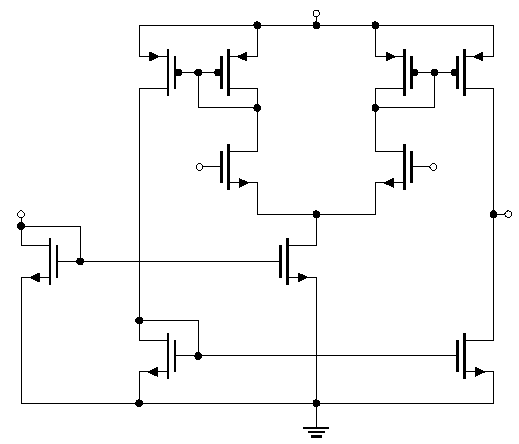
\includegraphics[width=0.65\linewidth]{Fig/SymmetricalOpAmp}
	\caption{Symmetrical op-amp} \label{fig:SymmetricalOpAmp}
\end{figure}

\begin{figure}[H]
	\centering
	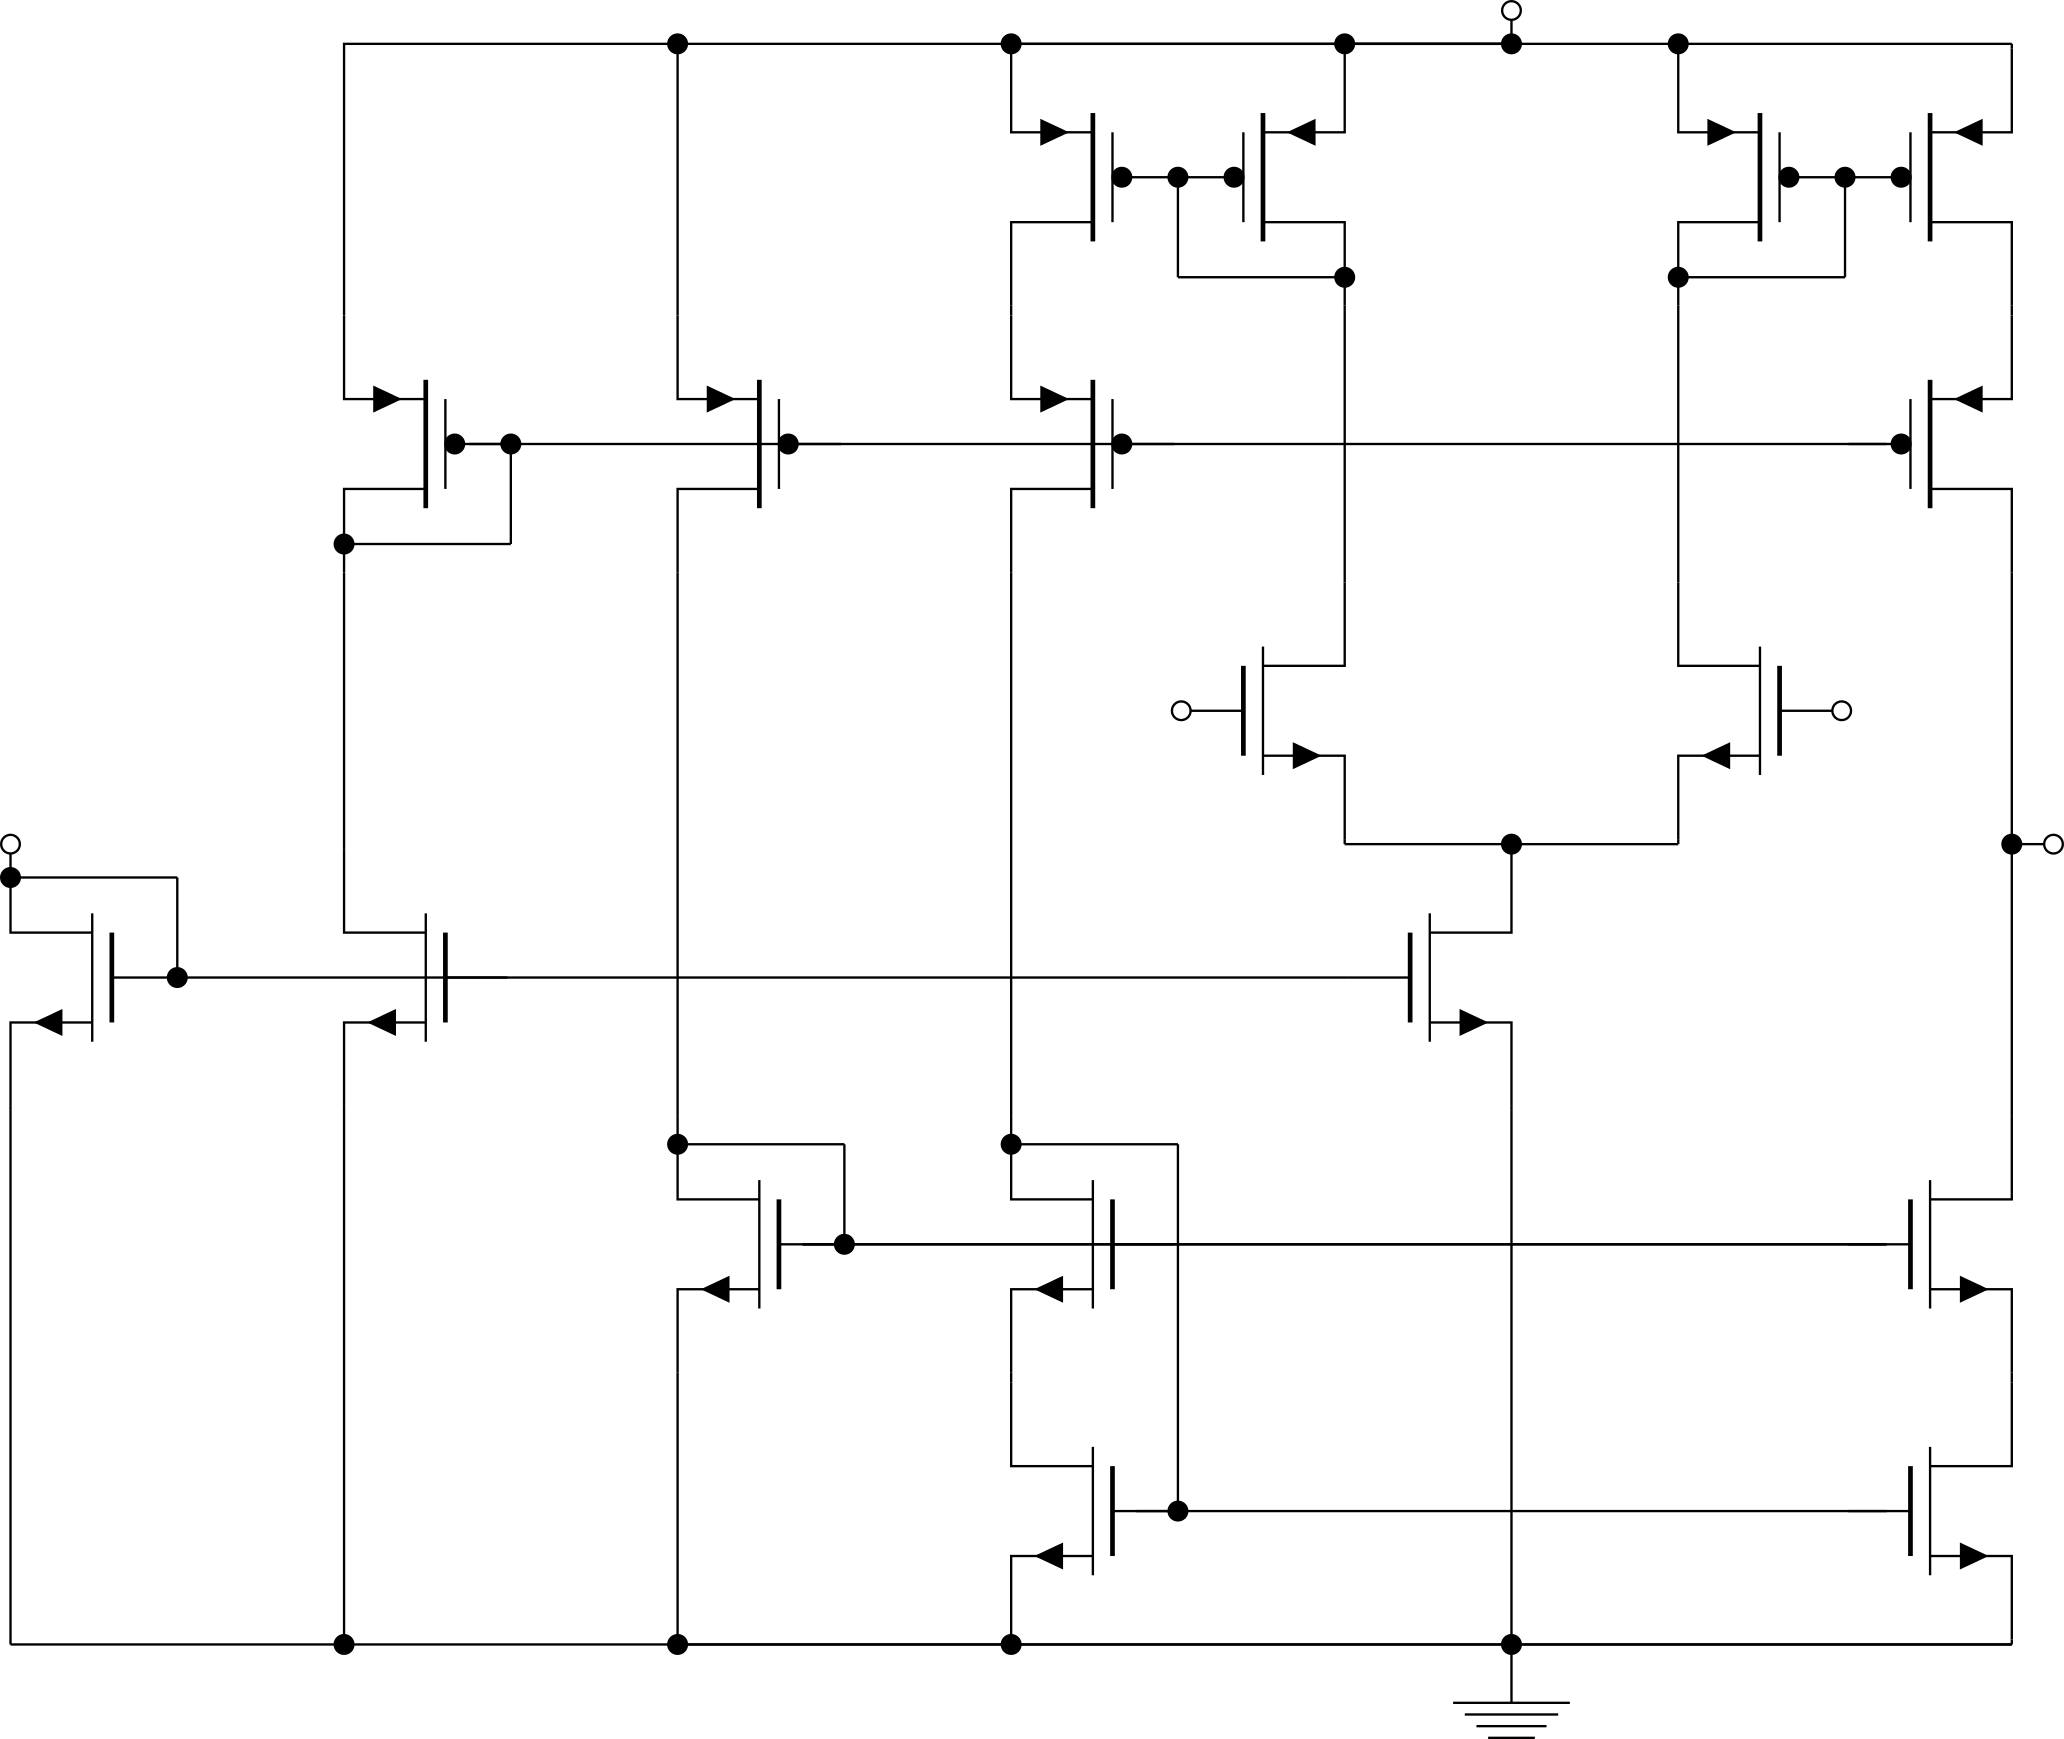
\includegraphics[width=\linewidth]{Fig/CascodeSymmetricalOTA.png}
	\caption{Cascode symmetrical op-amp} \label{fig:cascodeSymmetricalOpAmp}
\end{figure}

\begin{figure}[H]
	\centering
	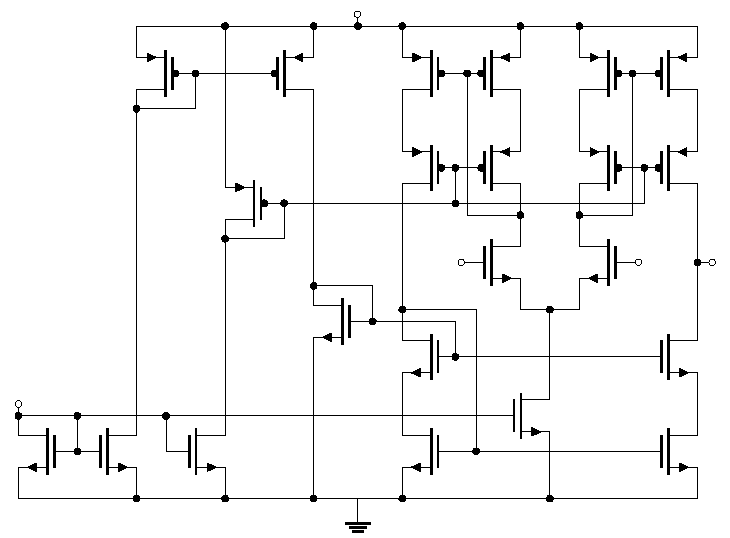
\includegraphics[width=0.8\linewidth]{Fig/SymmetricalOpAmp2}
	\caption{Cascode symmetrical op-amp with cascode first and second stage} \label{fig:SymmetricalOpAmp2}
\end{figure}

\begin{figure}[H]
	\centering
	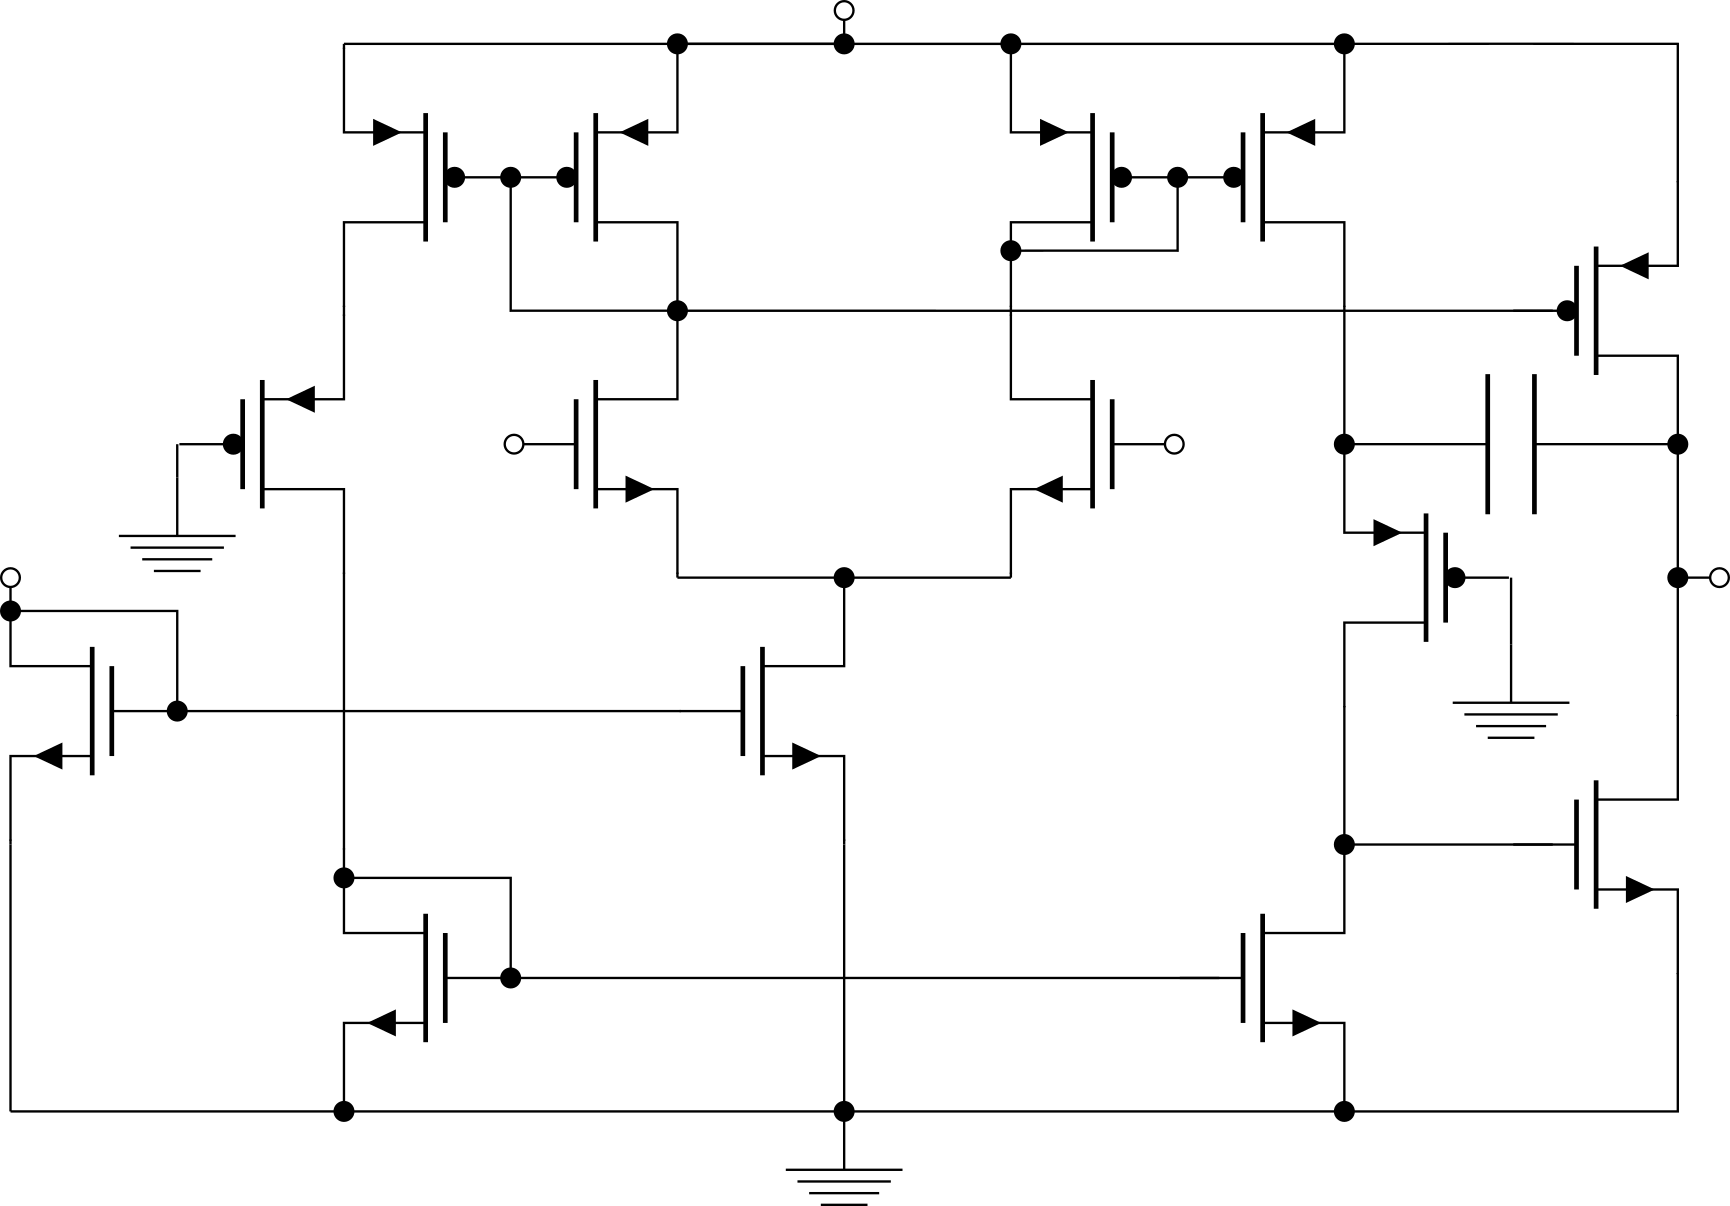
\includegraphics[width=0.7\linewidth]{Fig/SymmetricalOTAWithSecondStage.png}
	\caption{Symmetrical op-amp with high PSRR \cite{LakerSansen}} \label{fig:SymmetricalOpAmpWithHighPSRR}
\end{figure}




\section{Single-Output Op-Amps}

\begin{figure}[H]
	\centering
	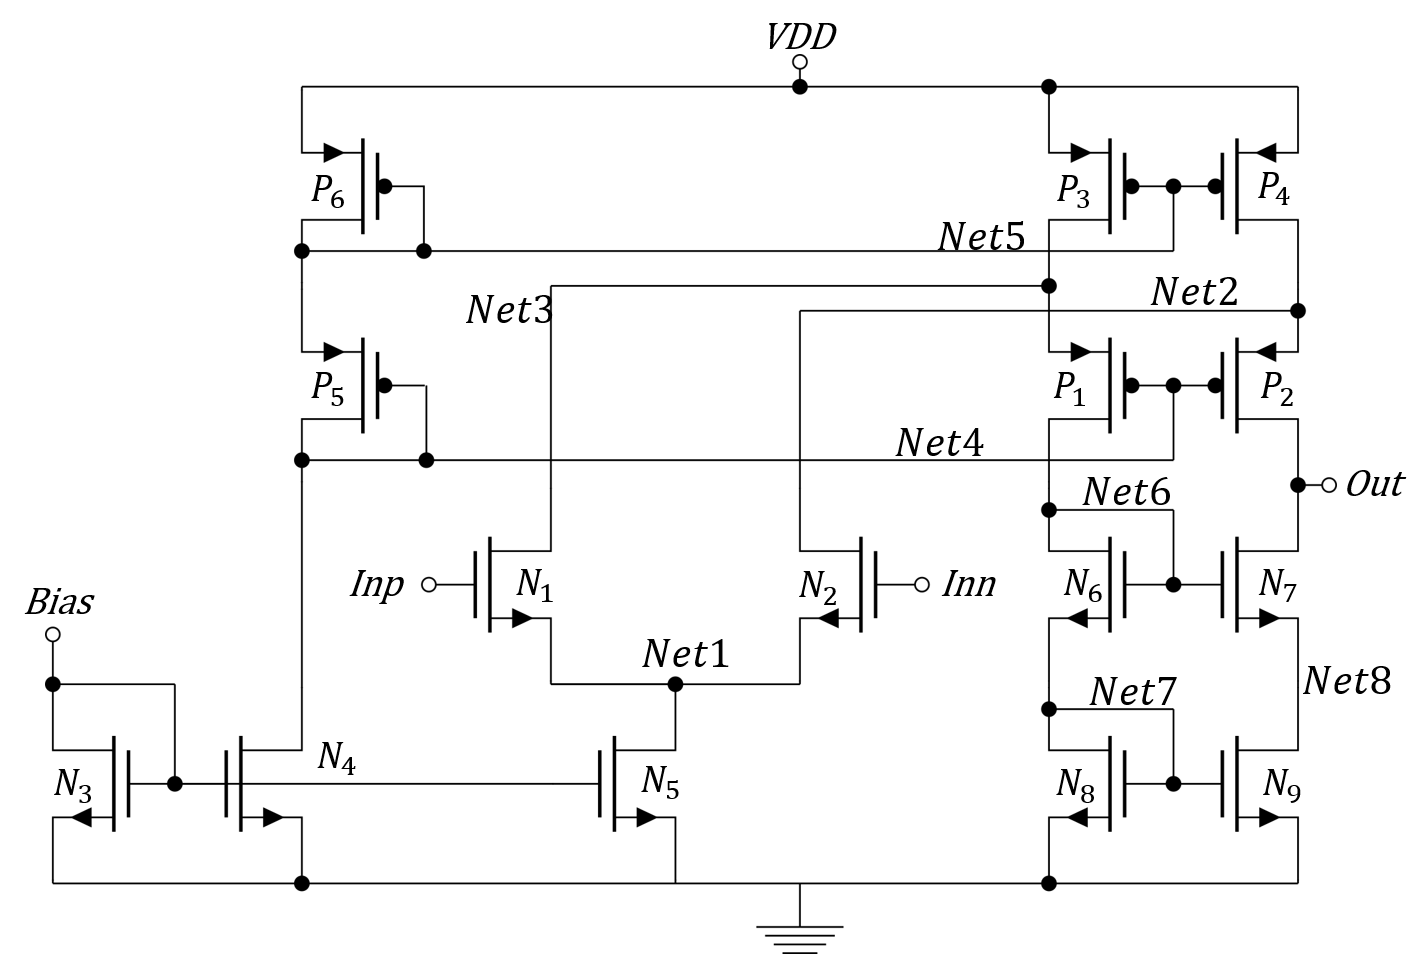
\includegraphics[width=0.75\linewidth]{Fig/foldedCascodeOpAmp.png}
	\caption{Folded-cascode op-amp with nmos differential stage} \label{fig:foldedCascodeOpAmpNMOS}
\end{figure}

\begin{figure}[H]
	\centering
	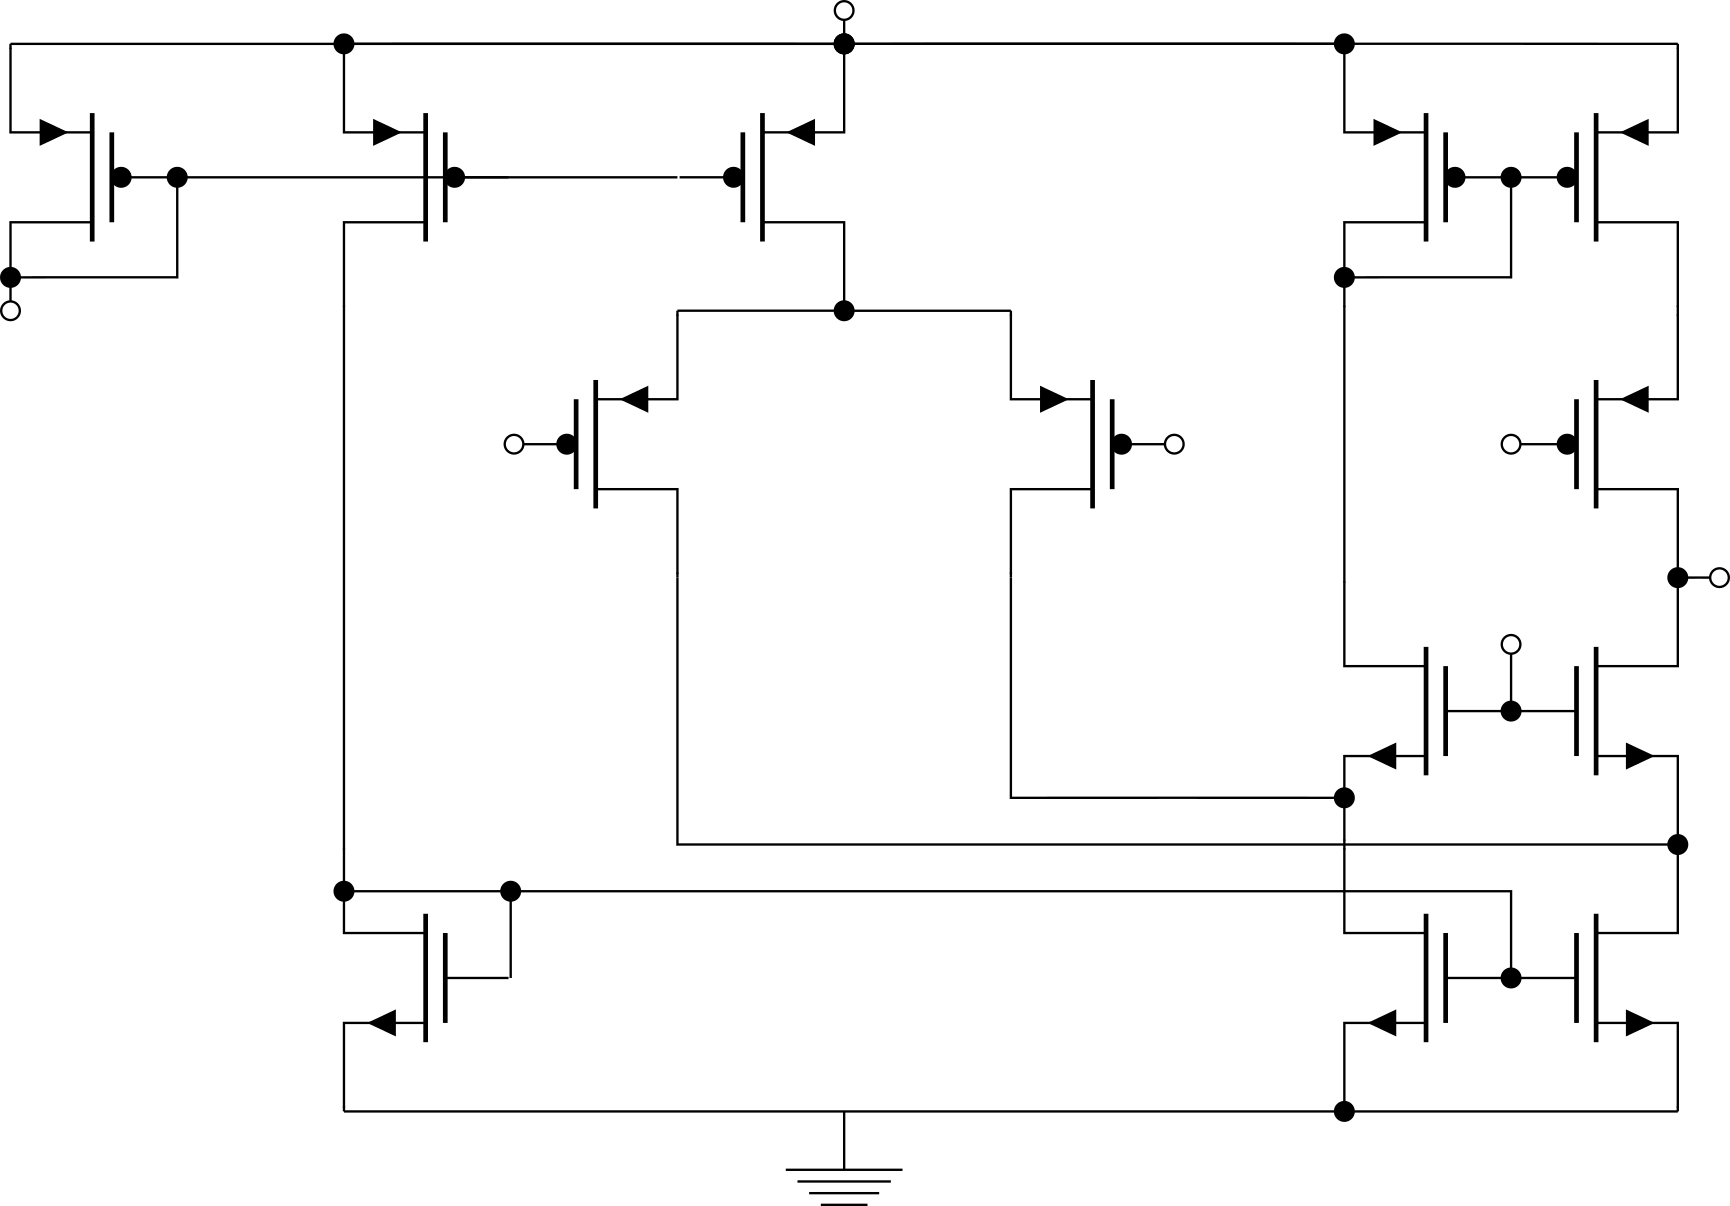
\includegraphics[width=0.7\linewidth]{Fig/FoldedCascodeOpAmpPmosDiffStage.png}
	\caption{Folded-cascode op-amp with pmos differential stage} \label{fig:foldedCascodeOpAmpPMOS}
\end{figure}

\begin{figure}[H]
	\centering
	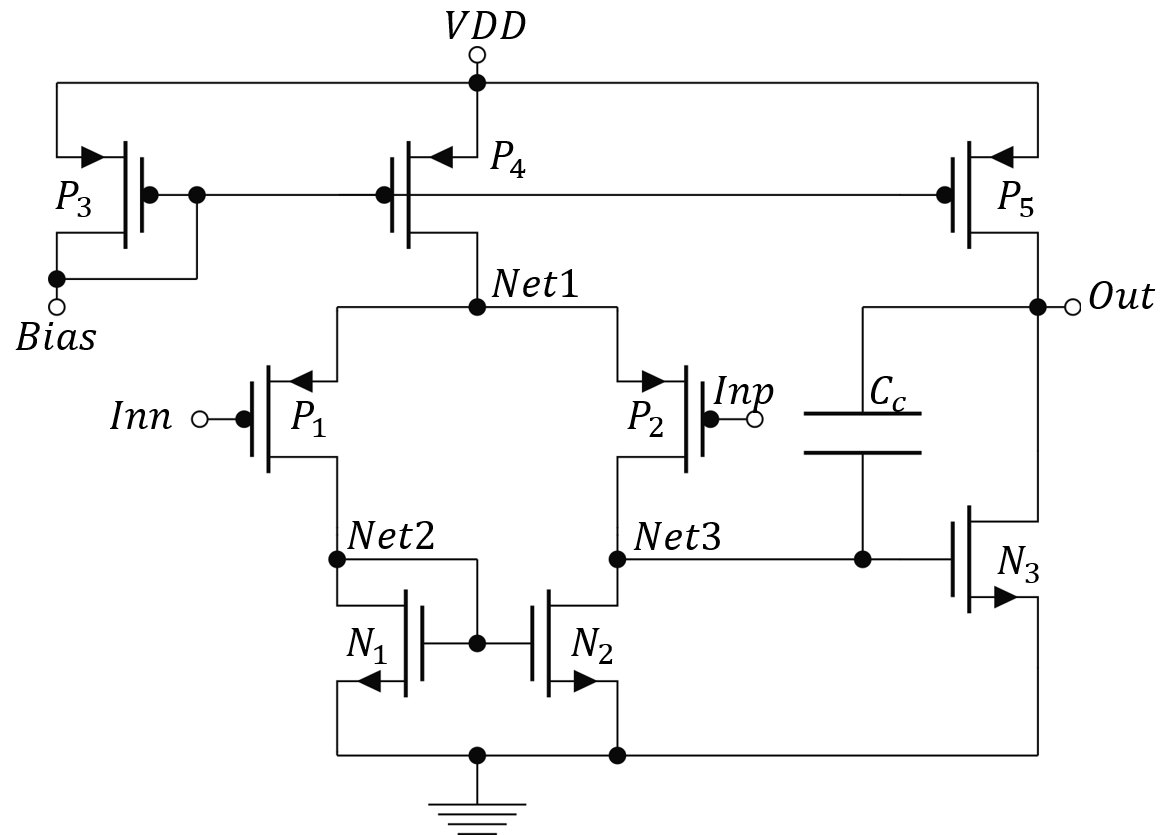
\includegraphics[width=0.65\linewidth]{Fig/Miller.png}
	\caption{Miller op-amp} \label{fig:MillerOpAmp}
\end{figure}

\begin{figure}[H]
	\centering
	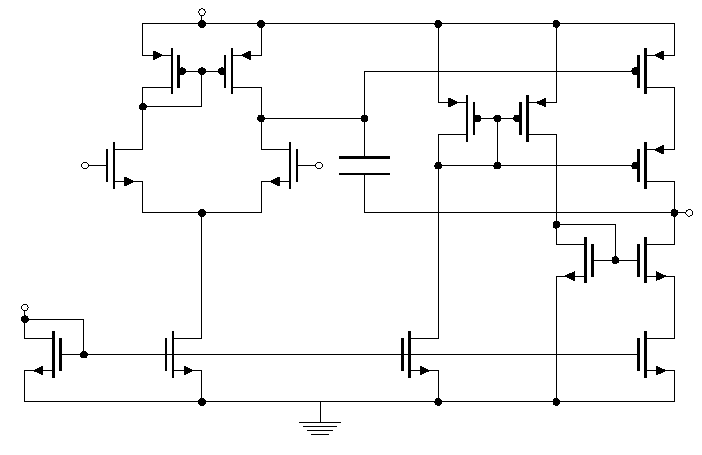
\includegraphics[width=0.8\linewidth]{Fig/TwoStageOpAmpWithCascodeSecondStage}
	\caption{Two-stage op-amp with cascode second stage} \label{fig:TwoStageOpAmpWithCascodeSecondStage}
\end{figure}

\begin{figure}[H]
	\centering
	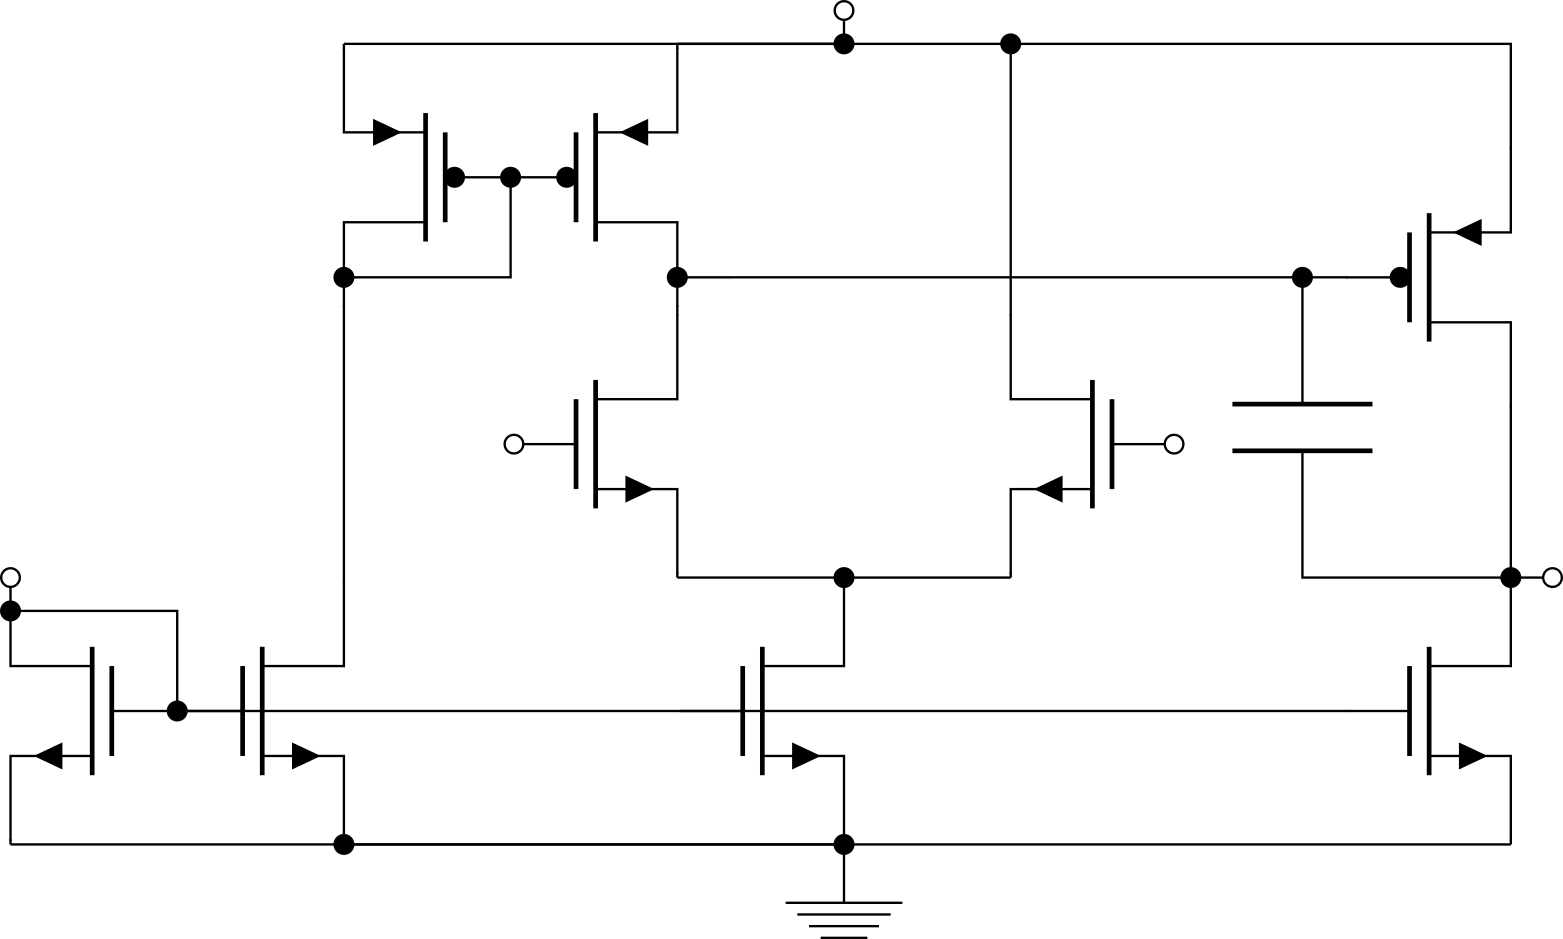
\includegraphics[width=0.6\linewidth]{Fig/TwoStageNMOSOpAmpWithOneLoadTransistor.PNG}
	\caption{Two-stage op-amp with one load transistor \cite{Allen}} \label{fig:TwoStageNMOSOpAmpWithOneLoadTransistor}
\end{figure}

\begin{figure}[H]
	\centering
	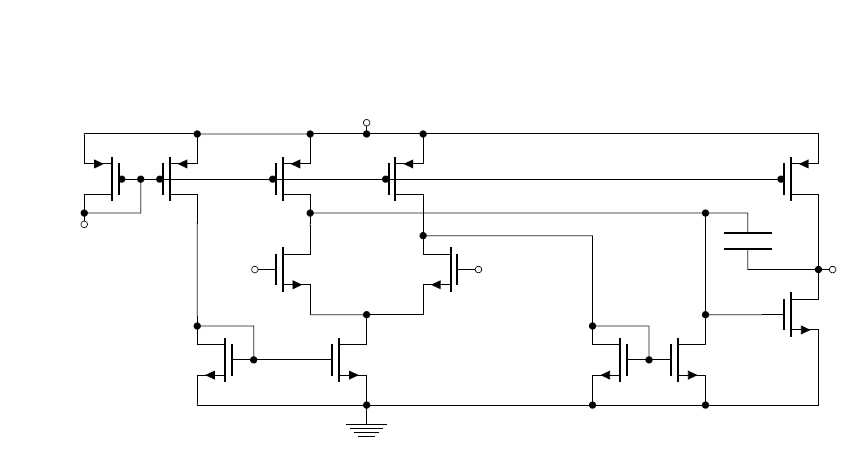
\includegraphics[width=0.9\linewidth]{Fig/LowPowerOpAmpWithTwoLoads.PNG}
	\caption{Low-power op-amp \cite{Allen}} \label{fig:lowPowerOpAmp}
\end{figure}

\begin{figure}[H]
	\centering
	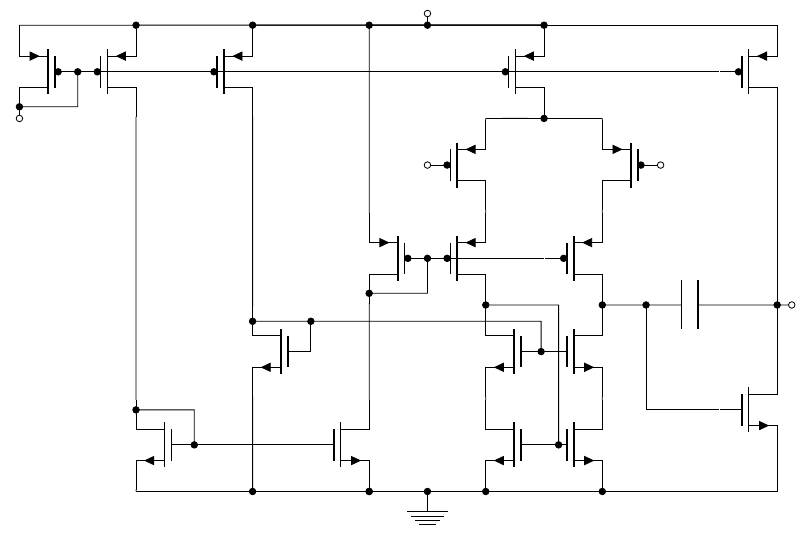
\includegraphics[width=0.9\linewidth]{Fig/OpAmpWithCascodeFirstStage.PNG}
	\caption{Telescopic op-amp} \label{fig:telescopicOpAmp1}
\end{figure}

\begin{figure}[H]
	\centering
	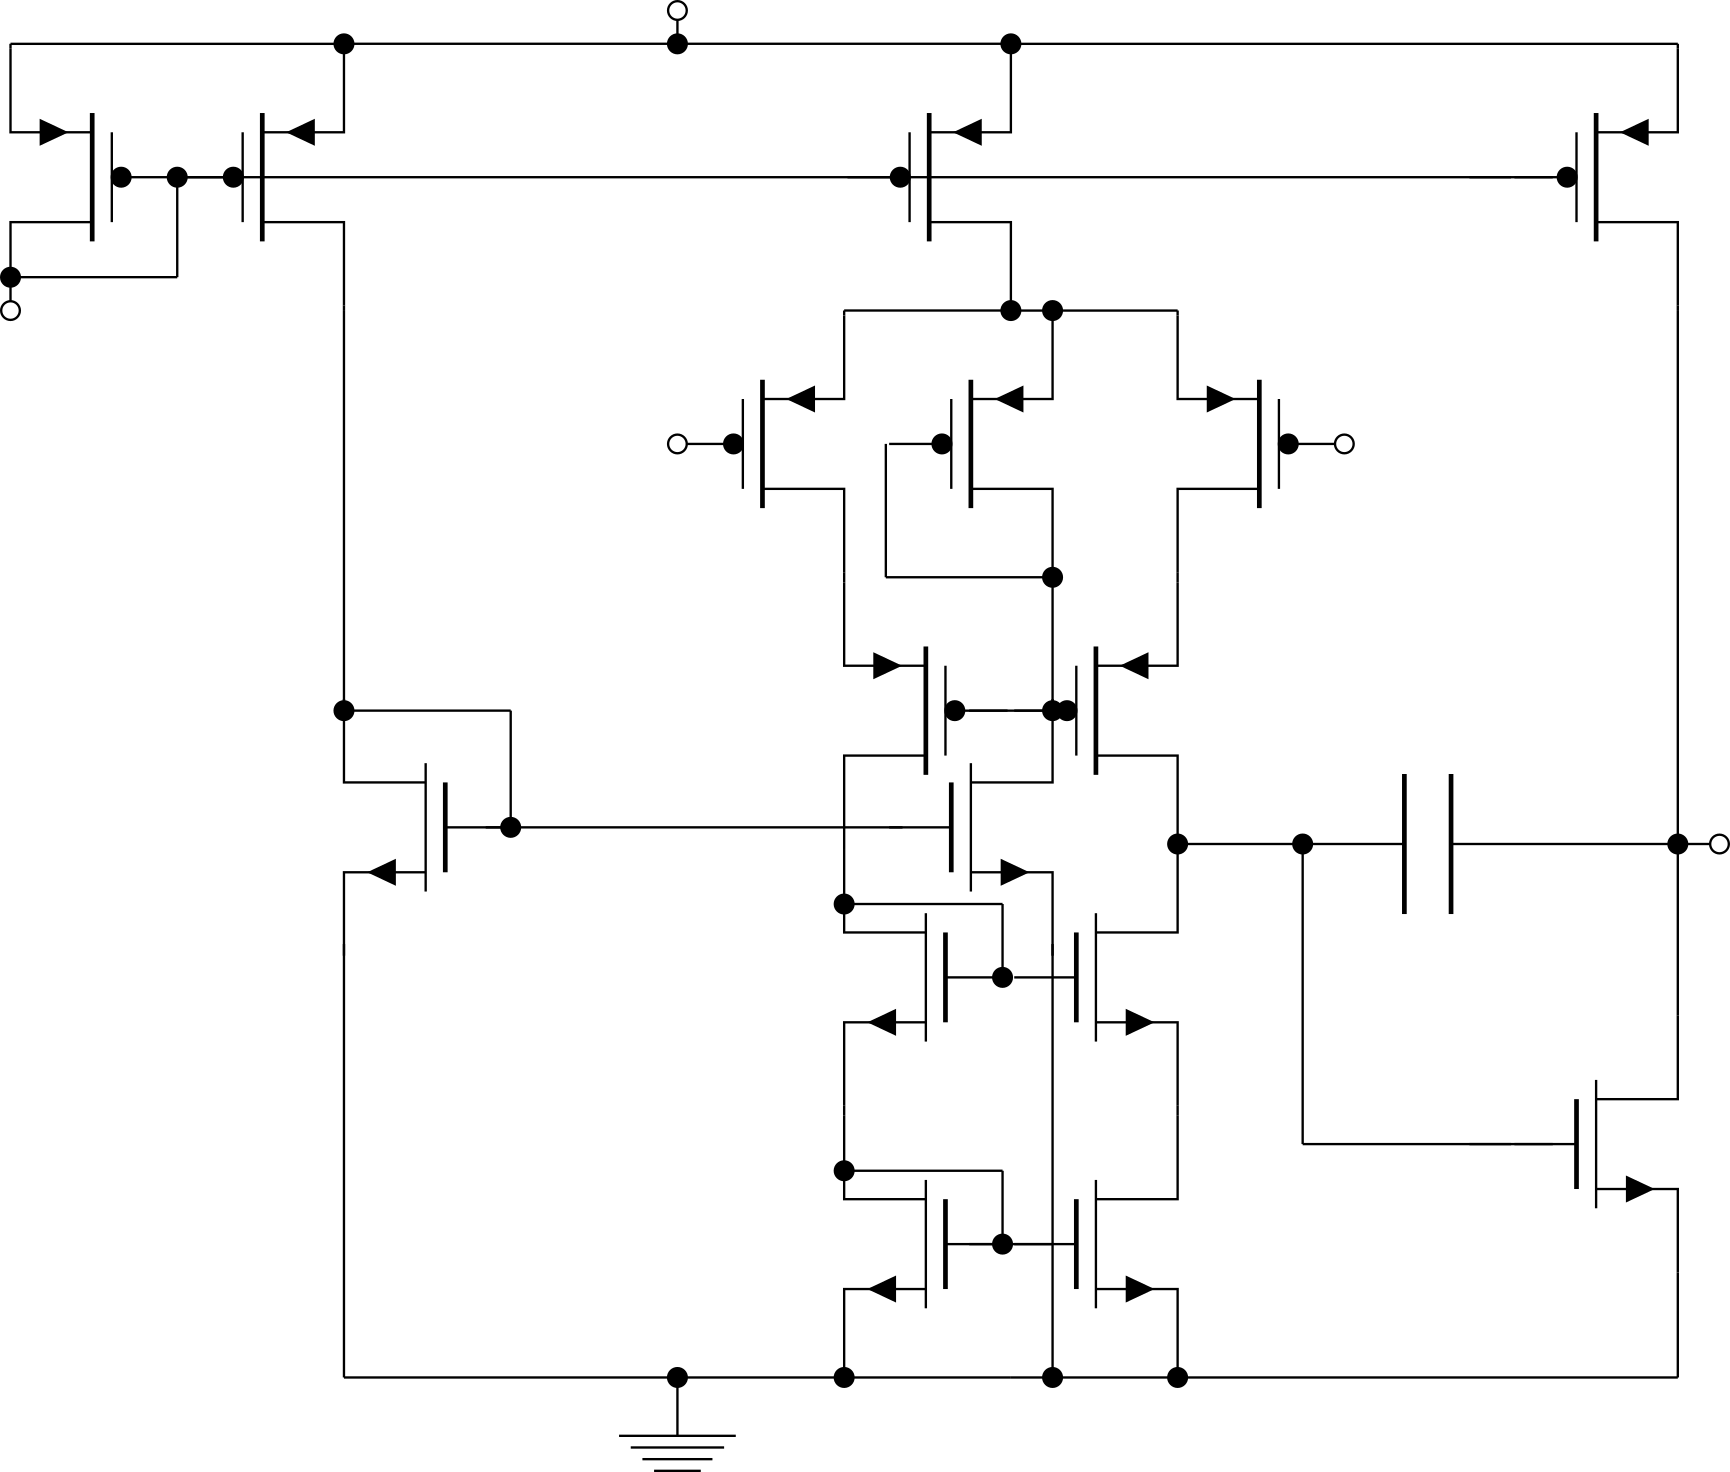
\includegraphics[width=0.7\linewidth]{Fig/OpAmpWitCascodeFirstStageInnerBias.PNG}
	\caption{Telescopic op-amp with different bias circuit} \label{fig:telescopicOpAmp2}
\end{figure}

\begin{figure}[H]
	\centering
	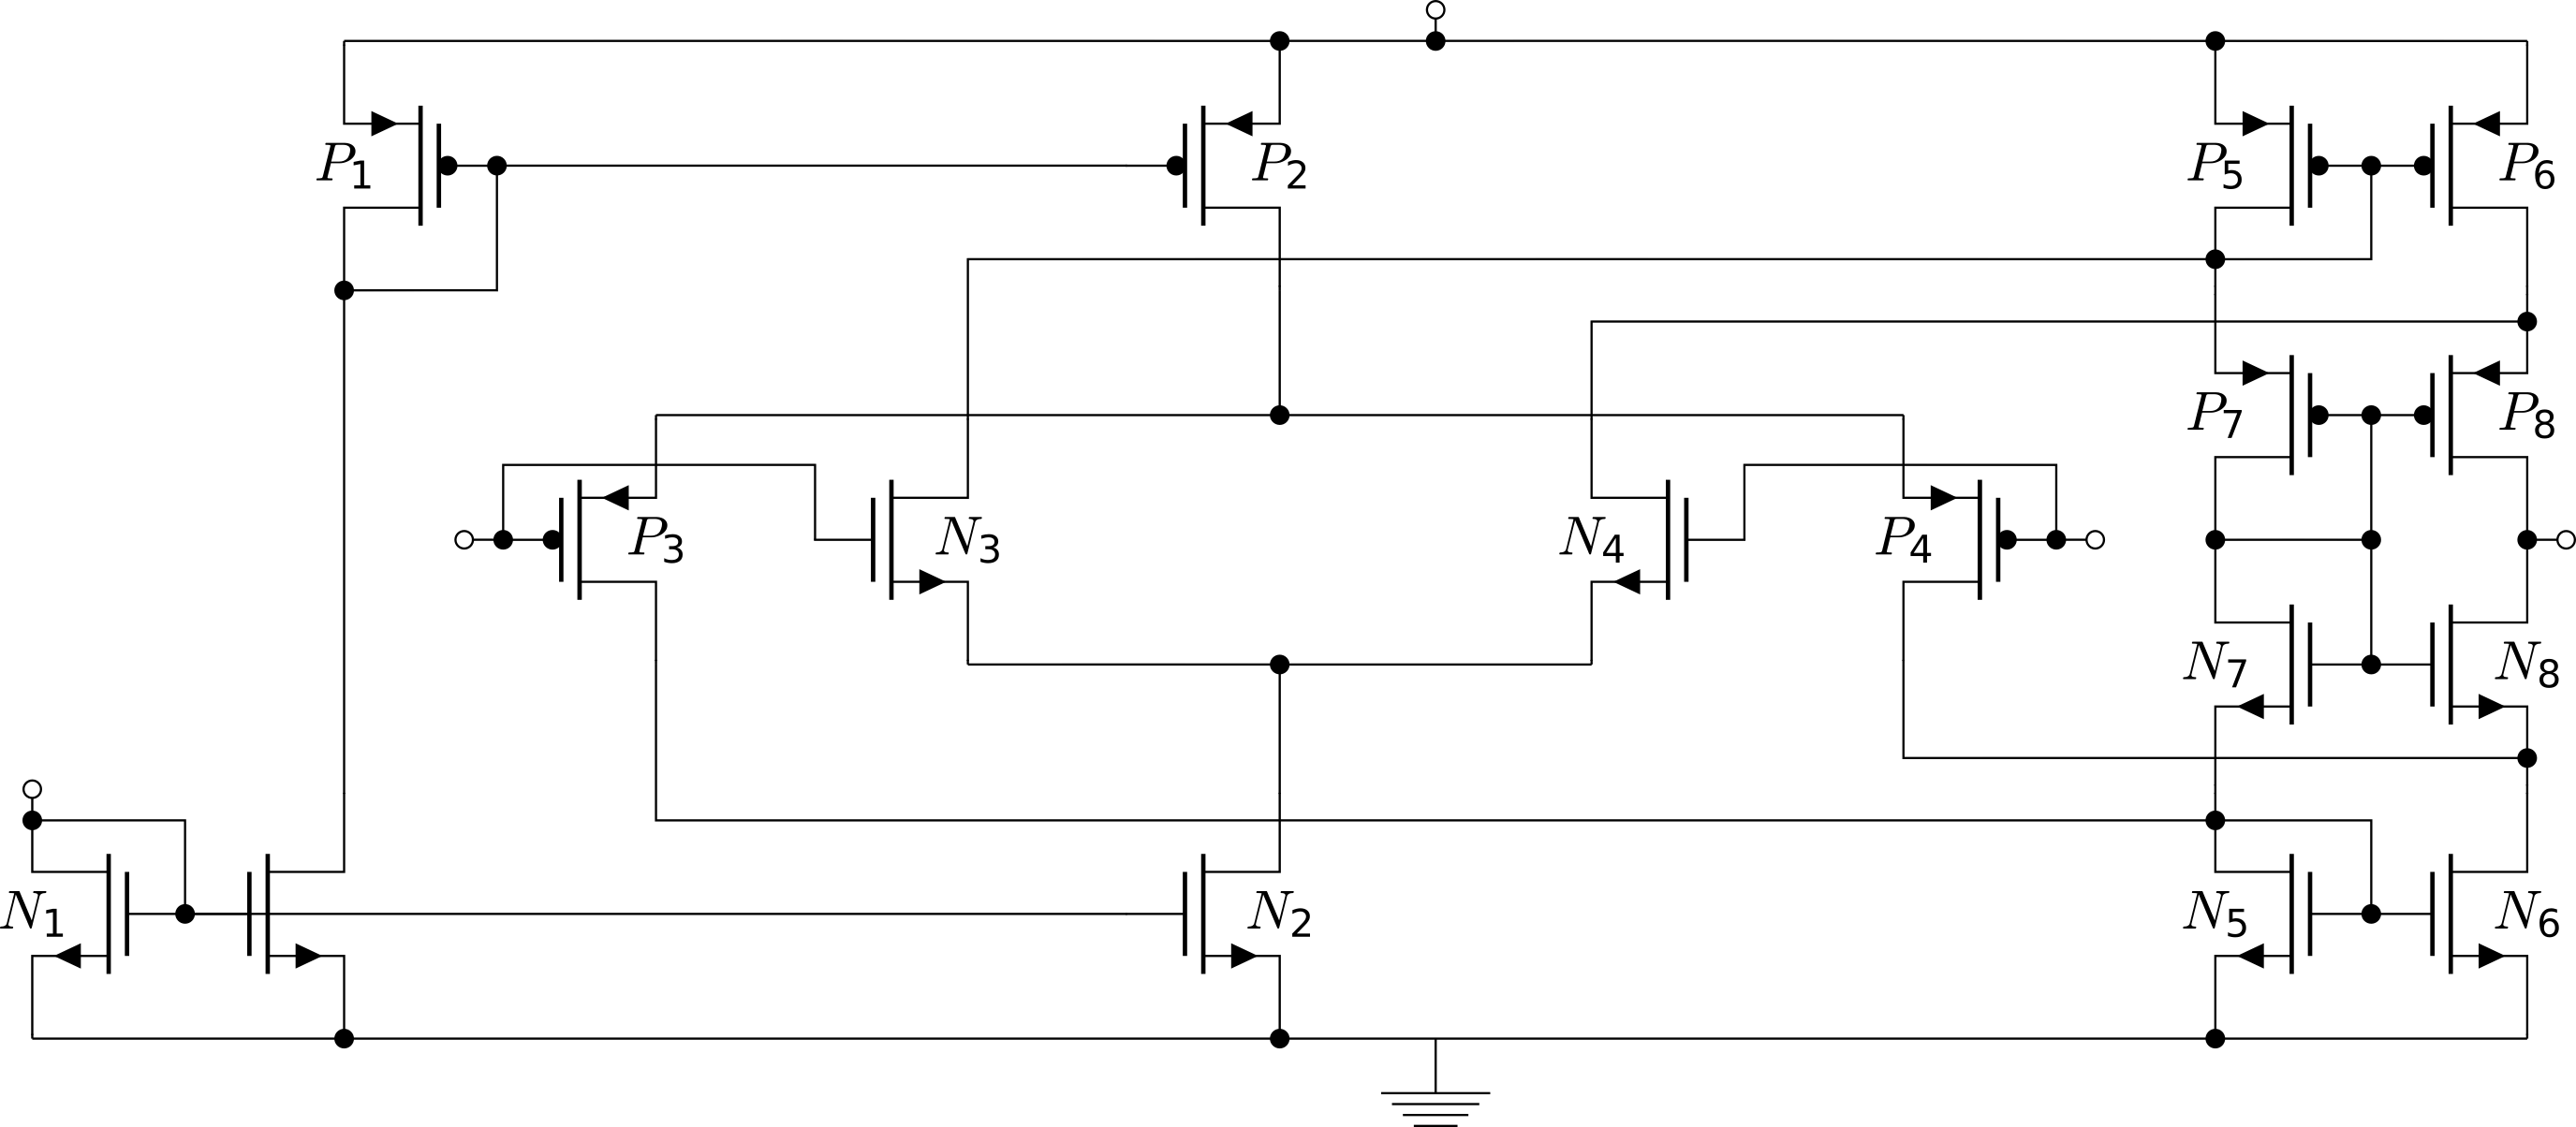
\includegraphics[width=\linewidth]{Fig/RailToRailAmplifier.PNG}
	\caption{Complementary op-amp} \label{fig:complementaryOpAmp2}
\end{figure}

\begin{figure}[H]
	\centering
	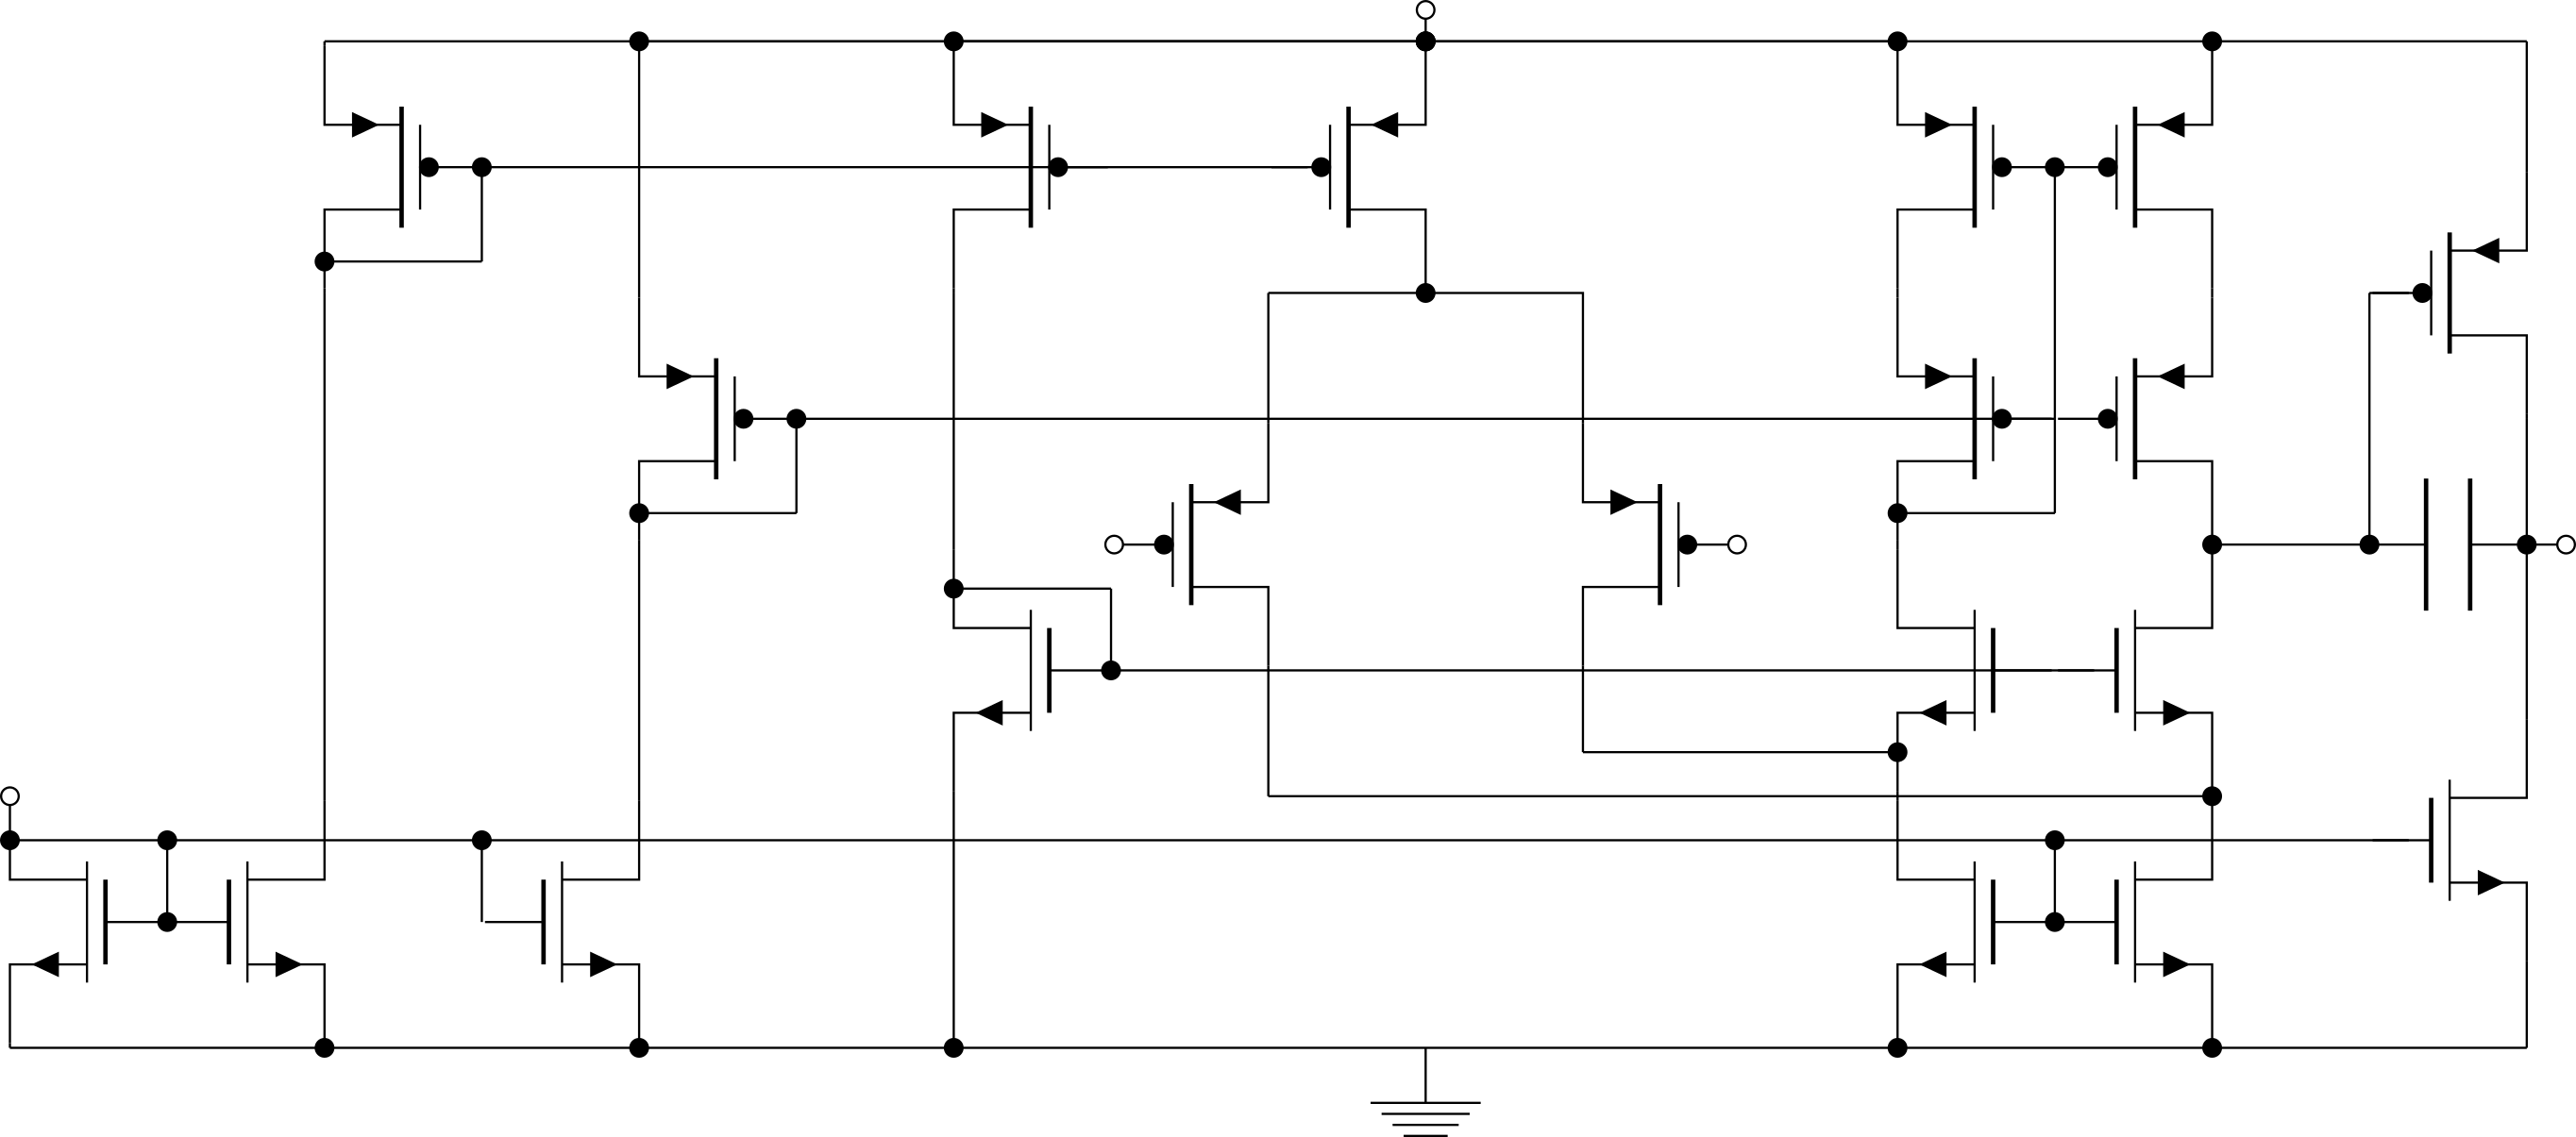
\includegraphics[width=\linewidth]{Fig/TwoStageFoldedCascodeOpAmp.PNG}
	\caption{Two-stage folded-cascode op-amp} \label{fig:twoStageFoldedCascodeOpAmp}
\end{figure}

\begin{figure}[H]
	\centering
	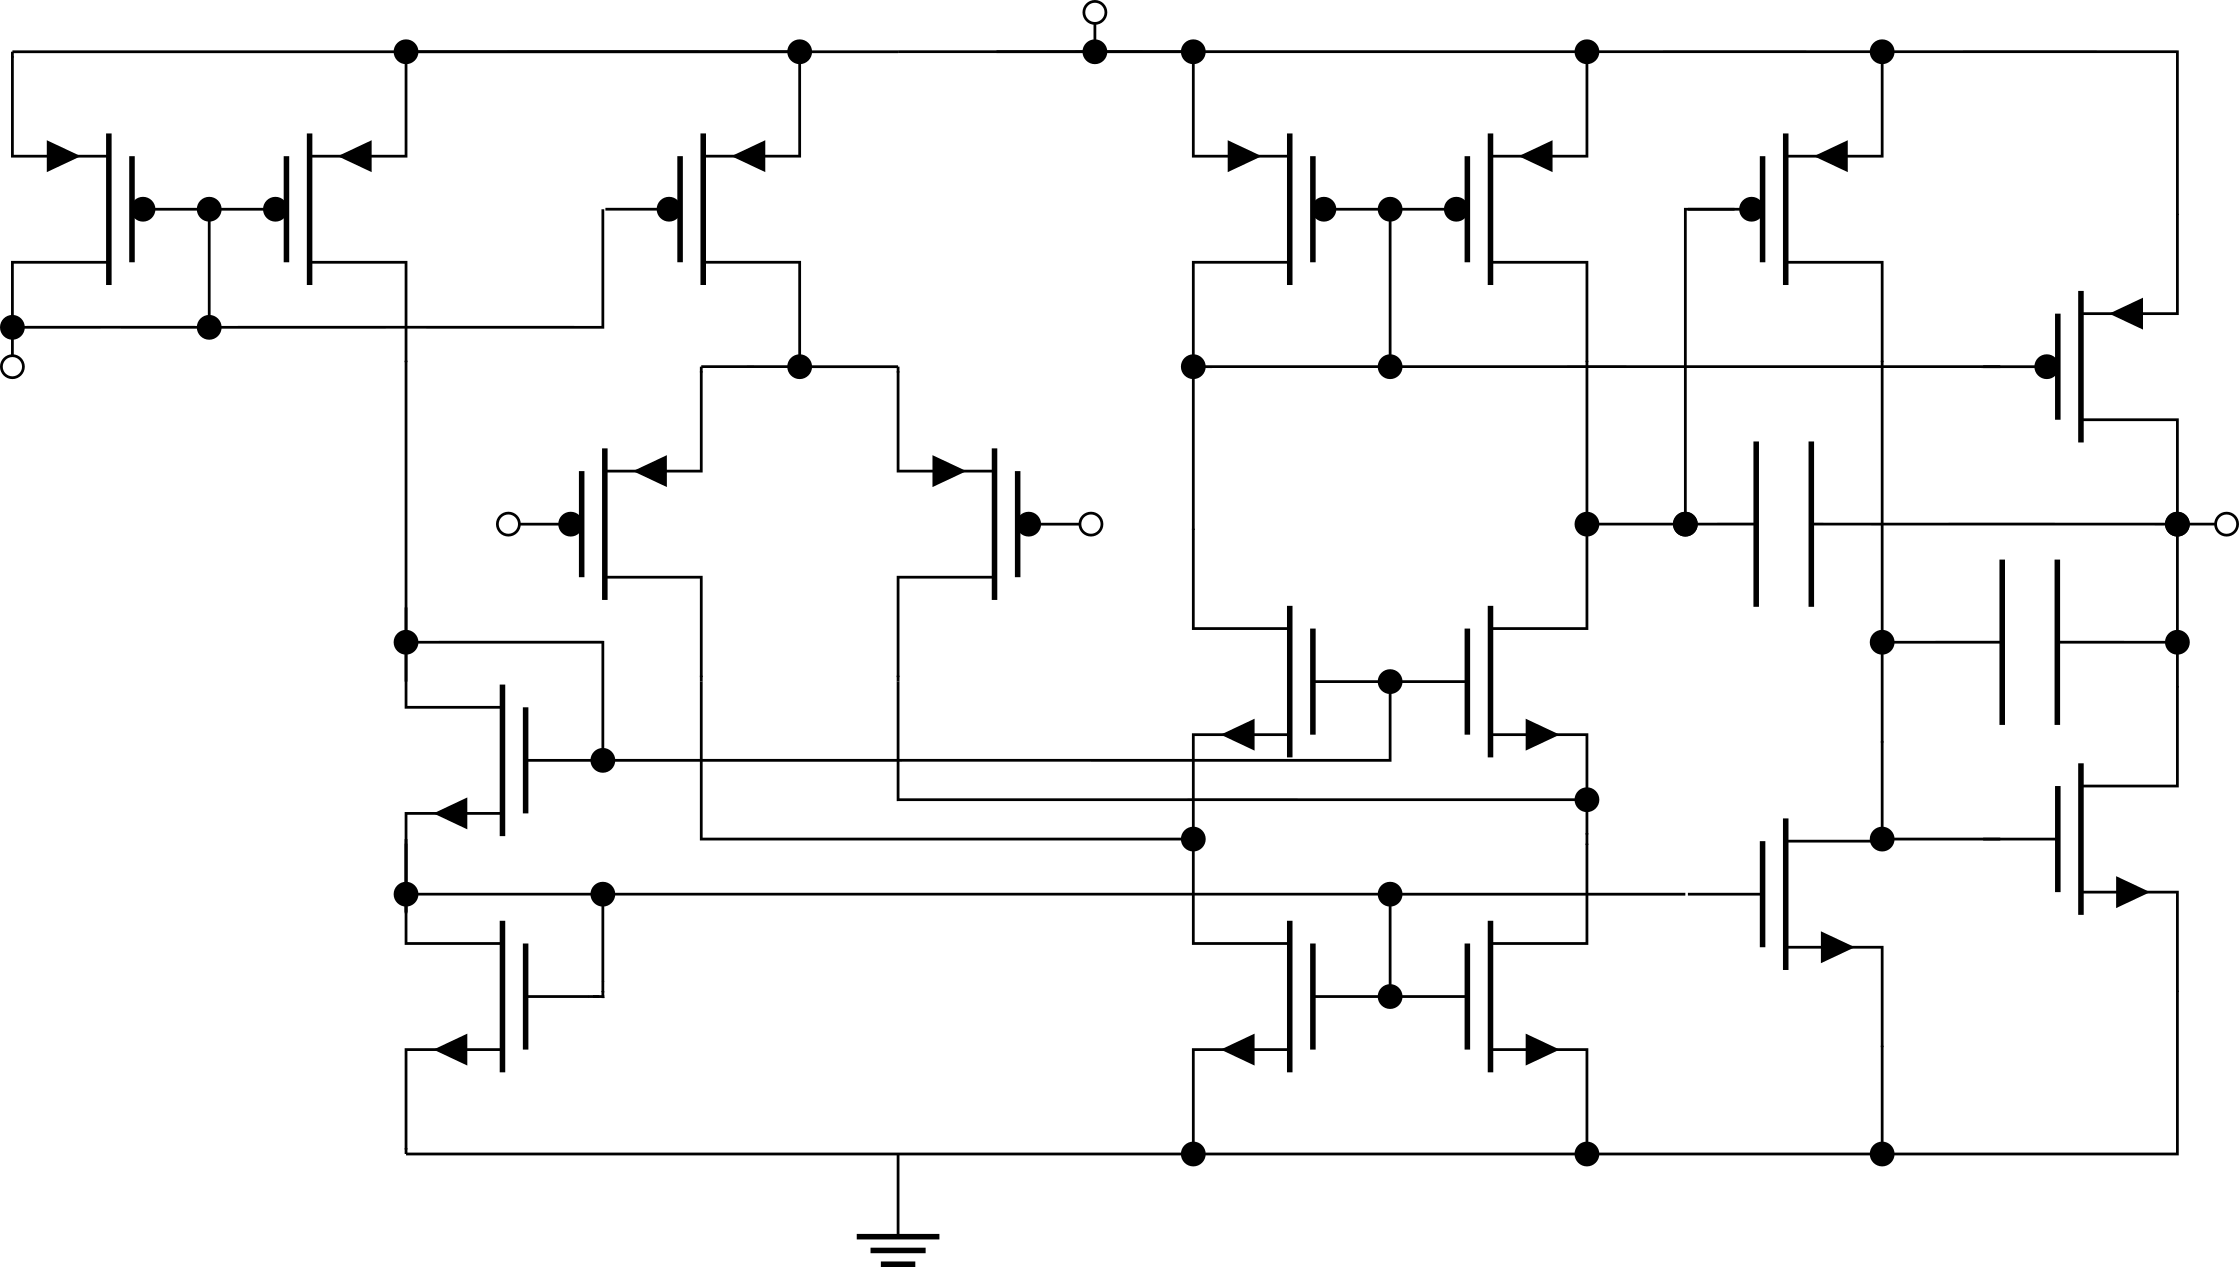
\includegraphics[width=0.8\linewidth]{Fig/ThreeStageOpAmp.PNG}
	\caption{Three-stage op-amp} \label{fig:threeStageOpAmp}
\end{figure}

\section{Fully-differential Op-Amps}

\begin{figure}[H]
	\centering
	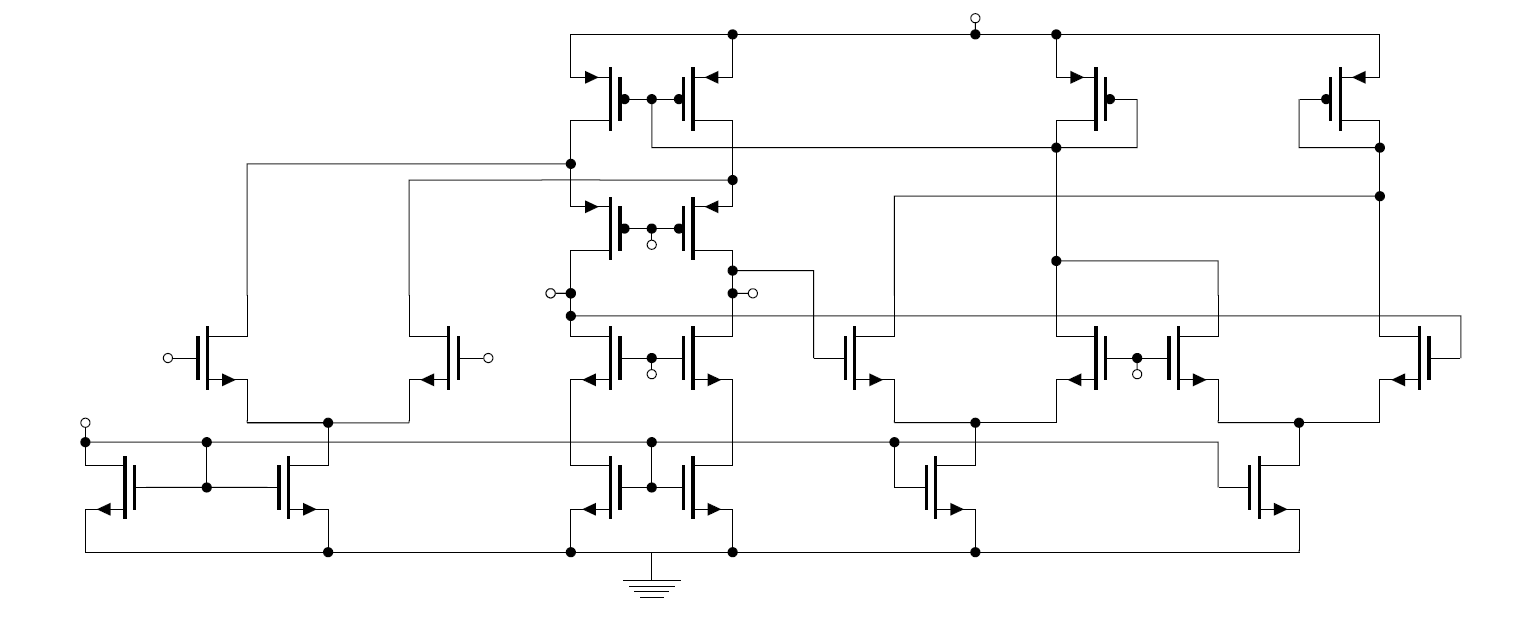
\includegraphics[width=\linewidth]{Fig/FoldedCascodeWithCMFB.png}
	\caption{Folded-cascode op-amp with CMFB stage} \label{fig:foldedCascodeOpAmpCMFB}
\end{figure}

\begin{figure}[H]
	\centering
	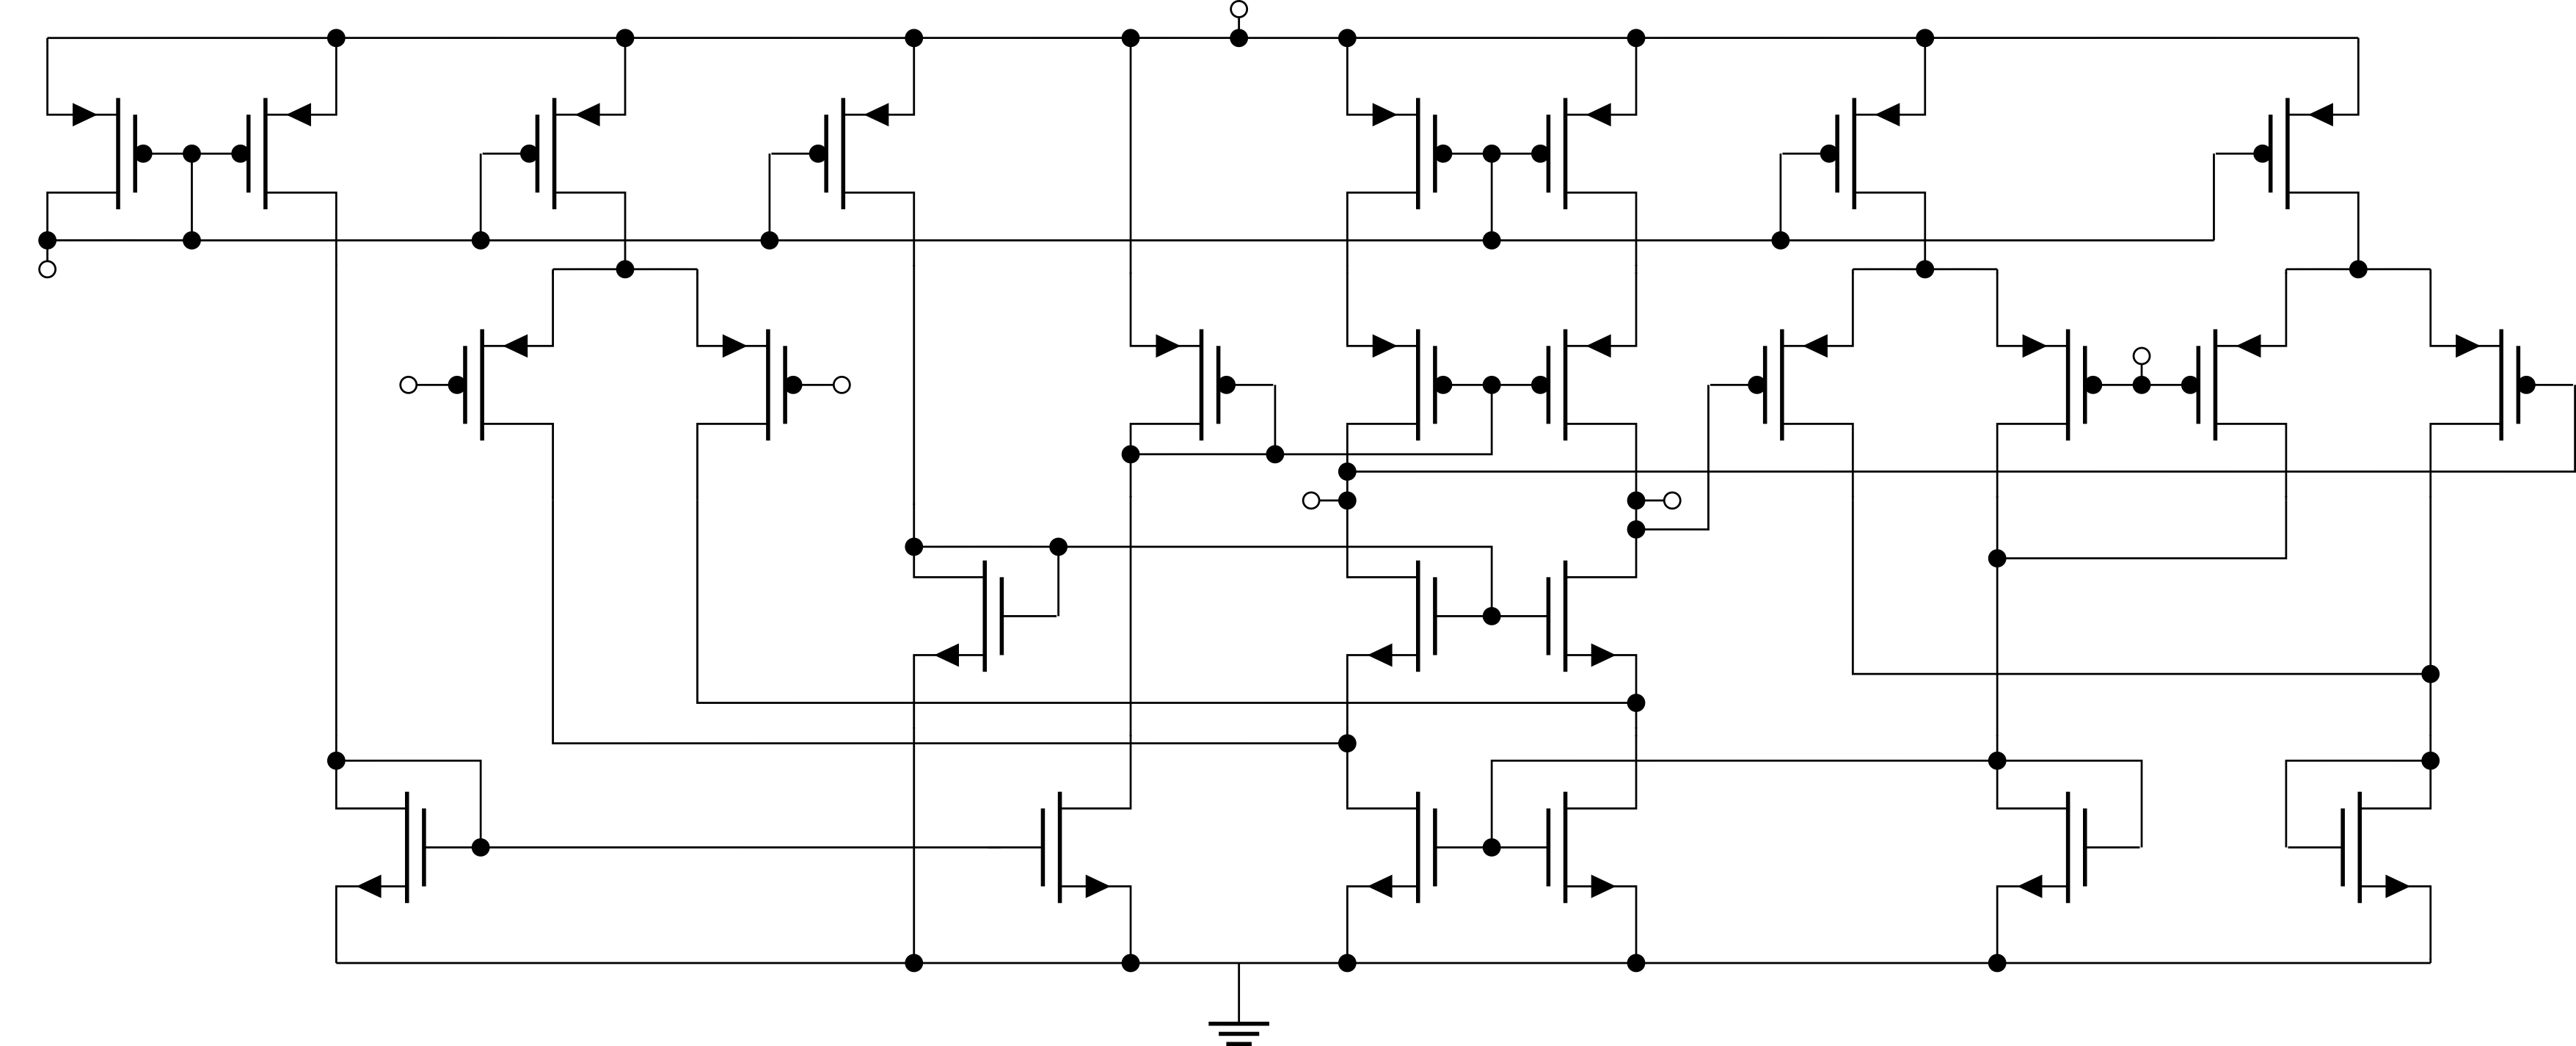
\includegraphics[width=\linewidth]{Fig/FoldedCascodeOpAmpWithCMFB.png}
	\caption{Folded-cascode op-amp with CMFB stage PMOS variant} \label{fig:foldedCascodeOpAmpCMFBPMOS}
\end{figure}

\chapter{Installation Guide for Supplementary Libraries Needed by acst}\label{ch:installationGuideSupplementaryLibraries}

The following installation guide does not claim to be complete and without errors. Please refer to the websites of the individual libraries for further information.

\section{Installation of Boost}
On most systems, Boost is already installed. You can check that with:
\begin{lstlisting}[basicstyle=\ttfamily\scriptsize,backgroundcolor={\color{gray!30}}, escapechar=!]
$ apt list --installed libboost-all-dev	
\end{lstlisting}
Or look at:
\begin{lstlisting}[basicstyle=\ttfamily\scriptsize,backgroundcolor={\color{gray!30}}, escapechar=!]
/usr/local/lib/cmake/
\end{lstlisting}

If it is not installed, you can download boost at \url{https://www.boost.org/} and install it with the following command in the directory of Boost:
\begin{lstlisting}[basicstyle=\ttfamily\scriptsize,backgroundcolor={\color{gray!30}}, escapechar=!]
$ ./bootstrap
$ ./b2
$ sudo ./b2 install
\end{lstlisting}




\section{Installation of RapidXml}
You can download RapidXml at \url{http://rapidxml.sourceforge.net/}.
No installation is needed. However, there is a bug in {\tt rapidxml\_print.hpp} if clang is used as compiler. You must add following lines to {\tt rapidxml\_print.hpp} as bug fix:
\begin{lstlisting}[basicstyle=\ttfamily\scriptsize,backgroundcolor={\color{gray!30}}, escapechar=!]
///////////////////////////////////////////////////////////////////////////
// Internal printing operations

//Predeclarations for bugfix
template<class OutIt, class Ch>
inline OutIt print_children(OutIt out, const xml_node<Ch> *node, int flags, int indent);

template<class OutIt, class Ch>
inline OutIt print_attributes(OutIt out, const xml_node<Ch> *node, int flags);

template<class OutIt, class Ch>
inline OutIt print_data_node(OutIt out, const xml_node<Ch> *node, int flags, int 
indent);

template<class OutIt, class Ch>
inline OutIt print_cdata_node(OutIt out, const xml_node<Ch> *node, int flags, int 
indent);

template<class OutIt, class Ch>
inline OutIt print_element_node(OutIt out, const xml_node<Ch> *node, int flags, int 
indent);

template<class OutIt, class Ch>
inline OutIt print_declaration_node(OutIt out, const xml_node<Ch> *node, int flags, int 
indent);

template<class OutIt, class Ch>
inline OutIt print_comment_node(OutIt out, const xml_node<Ch> *node, int flags, int 
indent);

template<class OutIt, class Ch>
inline OutIt print_doctype_node(OutIt out, const xml_node<Ch> *node, int flags, int 
indent);

template<class OutIt, class Ch>
inline OutIt print_pi_node(OutIt out, const xml_node<Ch> *node, int flags, int indent);
//Test for bugfix

// Print node
template<class OutIt, class Ch>
inline OutIt print_node(OutIt out, const xml_node<Ch> *node, int flags, int indent)
\end{lstlisting}


\section{Installation of GeCode}
For the correct installation of GeCode (\url{https://www.gecode.org/}) the GMP library (\url{https://gmplib.org/}) and  the MPFR (\url{https://www.mpfr.org/}) are needed, as they provide the needed support for trigonometrical and transcendental constraints.

On some systems, GMP and MPFR are preinstalled. You can check that by running the command {\tt ./configure} in the GeCode directory. Look at the output and check if gmp.h and mpfr.h was found. 

If they are not installed, download these libraries from the website and install them by using the commands:
\begin{lstlisting}[basicstyle=\ttfamily\scriptsize,backgroundcolor={\color{gray!30}}, escapechar=!]
$ ./configure
$ make
$ sudo make install
\end{lstlisting}
in their directory.

GMP depends on M4. If not already installed, you can install it with the following commands:
\begin{lstlisting}[basicstyle=\ttfamily\scriptsize,backgroundcolor={\color{gray!30}}, escapechar=!]
$ sudo apt-get update
$ sudo apt-get install m4
\end{lstlisting}

GeCode must be downloaded from the GeCode web page (\url{https://www.gecode.org/}). It is installed using the commands:
\begin{lstlisting}[basicstyle=\ttfamily\scriptsize,backgroundcolor={\color{gray!30}}, escapechar=!]
$ ./configure
$ make
\end{lstlisting}
in the GeCode directory.

